%%%%%%%%%%%%%%%%%%%% author.tex %%%%%%%%%%%%%%%%%%%%%%%%%%%%%%%%%%%
%
% sample root file for your "contribution" to a contributed volume
%
% Use this file as a template for your own input.
%
%%%%%%%%%%%%%%%% Springer %%%%%%%%%%%%%%%%%%%%%%%%%%%%%%%%%%


% RECOMMENDED %%%%%%%%%%%%%%%%%%%%%%%%%%%%%%%%%%%%%%%%%%%%%%%%%%%
\documentclass[graybox]{svmult}

% choose options for [] as required from the list
% in the Reference Guide

\usepackage{type1cm}        % activate if the above 3 fonts are
                            % not available on your system
%
\usepackage{makeidx}         % allows index generation
\usepackage{graphicx}        % standard LaTeX graphics tool
                             % when including figure files
\usepackage{multicol}        % used for the two-column index
\usepackage[bottom]{footmisc}% places footnotes at page bottom


\usepackage{newtxtext}       % 
\usepackage{newtxmath}       % selects Times Roman as basic font

\usepackage{booktabs}       %Booktabs Table Style


% see the list of further useful packages
% in the Reference Guide

\makeindex             % used for the subject index
                       % please use the style svind.ist with
                       % your makeindex program

%%%%%%%%%%%%%%%%%%%%%%%%%%%%%%%%%%%%%%%%%%%%%%%%%%%%%%%%%%%%%%%%%%%%%%%%%%%%%%%%%%%%%%%%%

\DeclareUnicodeCharacter{2212}{-}
\DeclareUnicodeCharacter{22C5}{-}

\begin{document}

\title*{Recovering from population extinction in the Animal Life Cycle Algorithm (ALCA)} 
\titlerunning{Animal Life Cycle Algorithm (ALCA)}
% Use \titlerunning{Short Title} for an abbreviated version of
% your contribution title if the original one is too long
\author{J. C. Felix-Saul, Mario García Valdez}
% Use \authorrunning{Short Title} for an abbreviated version of
% your contribution title if the original one is too long
\institute{J. C. Felix-Saul \at Tijuana Institute of Technology, Tijuana, Mexico, \email{name@email.address}
\and Mario García Valdez \at Tijuana Institute of Technology, Tijuana, Mexico, \email{name@email.address}}
%
% Use the package "url.sty" to avoid
% problems with special characters
% used in your e-mail or web address
%
\maketitle

\abstract*{In previous work, we introduced an algorithm inspired by the
biological Life Cycle of animal species, consisting of the stages: birth,
growth, reproduction, and death. As in nature, population individuals grow
older and age. In this algorithm's reproduction process, couples must match by
mutual attraction, where sometimes individuals won't procreate offspring
because of the mate's low appeal. As time passes, the environment kills its
individuals either because of low fitness or age, causing occasional population
extinction. When this condition presents, it is required to create a new
population if evaluations are available and termination conditions are
favorable to continue. Some alternatives we explored to restart this new
population are the random generation of a new set of candidate solutions and
the creation of a new set of candidate solutions based on either: a mix of
elements from the best historically found candidate solutions set (Elite); the
mutation with uniform modification from the Elite or the historically
best-found solution (Champion); crossing the Champion with the Elite; the
projection of the Elite towards the Champion; based on random use of the
previous alternatives. In this paper, we present one of the most promising
alternatives to solve population extinction caused by nature's pressure in the
Life Cycle algorithm: the projection of the Elite towards the Champion, where
we compare the results obtained with the latter and the random use of all the
alternatives, using classic benchmark functions for optimization for
comparison.}

\abstract{In previous work, we introduced an algorithm inspired by the
biological Life Cycle of animal species, consisting of the stages: birth,
growth, reproduction, and death. As in nature, population individuals grow
older and age. In this algorithm's reproduction process, couples must match by
mutual attraction, where sometimes individuals won't procreate offspring
because of the mate's low appeal. As time passes, the environment kills its
individuals either because of low fitness or age, causing occasional population
extinction. When this condition presents, it is required to create a new
population if evaluations are available and termination conditions are
favorable to continue. Some alternatives we explored to restart this new
population are the random generation of a new set of candidate solutions and
the creation of a new set of candidate solutions based on either: a mix of
elements from the best historically found candidate solutions set (Elite); the
mutation with uniform modification from the Elite or the historically
best-found solution (Champion); crossing the Champion with the Elite; the
projection of the Elite towards the Champion; based on random use of the
previous alternatives. In this paper, we present one of the most promising
alternatives to solve population extinction caused by nature's pressure in the
Life Cycle algorithm: the projection of the Elite towards the Champion, where
we compare the results obtained with the latter and the random use of all the
alternatives, using classic benchmark functions for optimization for
comparison.}

%\keywords{Distributed Bioinspired Algorithms \and Genetic Algorithms \and Cloud Computing.}

\newpage
\section{Introduction}
\label{sec:1}

Bio-inspired algorithms have been very successful when used to solve complex
optimization problems
\cite{castillo2019comparative,valdez2021swarm,acherjee2020ultrasonic}, but as
their complexity increases so does the computing power required to execute them
\cite{ontiveros2018high}. One strategy to address this processing need is to
use distributed computing \cite{thain2005distributed}, or the resources
available in the cloud to help find the solution
\cite{garcia2013there,eshratifar2019bottlenet}. This strategy gives us
elasticity to increase (or reduce) the computing power to achieve a balance
according to the nature of the problem.

Most bio-inspired algorithms are traditionally designed with a sequential
(synchronous) perspective \cite{porto2018evolutionary,back1996evolutionary},
where each process must wait for the previous task to finish before continuing.
Our proposal presents an algorithm in its entirety as a native solution in the
cloud, fully distributed, where its processes are executed in parallel and
asynchronously. We designed the algorithm as a cloud-native solution using the
cloud available resources to divide the processing workload, among several
computers or running the algorithm as a cloud service. This technique makes it
easy to scale the computing power according to the complexity required by the
problem \cite{armbrust2010view}.

In previous work, we introduced an algorithm inspired by the biological
life-cycle of animal species. As in nature, population individuals grow older
and age. In this algorithm's reproduction process, couples must match by mutual
attraction, where sometimes individuals won't procreate offspring because of
the mate's low appeal. As time passes, the environment kills its individuals
either because of low fitness or age, causing occasional population extinction.
When this condition presents itself, it is required to create a new population
to continue evolution (restart). We previously used to generate a new random
set of solutions, with the cost of losing all evolution knowledge.

The main contribution of this paper is to demonstrate that it is possible to
evolve a population of individuals, similar to a Genetic Algorithm (GA), using
a distributed, parallel, and asynchronous methodology by algorithm
implementation and testing. We improve the algorithm behavior by solving
population extinction caused by nature's pressure in the Animal Life Cycle
Algorithm with one of the most promising alternatives: the projection of the
Elite towards the Champion, where we compare the results obtained with the
latter and the random use of the more traditional alternatives (mutation and
crossover), using classic benchmark functions for optimization for comparison.

We present the description of the following sections in our paper. First, we
illustrate our algorithm model, the encountered problem with the occasional
population extinction, and our proposed solution in
section~\ref{section.proposal}, followed by our experimental configuration and
results in section~\ref{section.experiments}, where we continue to analyze and
describe some of our research findings in section~\ref{section.discussion}. We
finalize by presenting some inferences based on the results of our experiments
in section~\ref{section.conclusions}.


\section{Proposal}
\label{section.proposal}
% Always give a unique label
% and use \ref{<label>} for cross-references
% and \cite{<label>} for bibliographic references
% use \sectionmark{}
% to alter or adjust the section heading in the running head

Our inspiration for this algorithm was found in the study and observation of
nature, using general abstraction to identify what most animal species have in
common: the life cycle. We present an algorithm inspired by the biological
life-cycle of animal species, which consists of several stages
\cite{read1968system}: birth, growth, reproduction, and death. The combination
of those processes results in evolution. As in nature, we intend to execute all
these stages in parallel and asynchronously on a constantly evolving
population.

\subsection{Algorithm Model}

This algorithm seeks to imitate the natural life cycle, where new individuals
are born at any moment and mature over time, where they age and then suffer
mutations throughout their lives. In reproduction, couples match by mutual
attraction. Death can happen to everyone: from a newborn to an aged adult,
where the individual's fitness will impact their longevity. We display the
general model concept in Figure~\ref{fig.algorithm_model}.

\subsubsection{Birth} Birth is the first process of our algorithm, and it is
responsible for the initial generation of individuals. This algorithm starts
with a randomly generated population.

\subsubsection{Growth} As in nature, all individuals constantly grow, mature,
or age. With increasing age, individuals may lose strength but may also gain
knowledge to solve problems. We represent this with a possible mutation in each
increment of age.

\subsubsection{Reproduction} This process will select random pairs of
individuals to evaluate their attraction as a couple, where this attraction
will depend on fitness. The better individual's fitness, the more attractive it
will be. Not all couples will be compatible, so reproduction will not always be
possible. When the breeding is successful, a new pair of individuals will be
born (offspring).

\subsubsection{Death} The death stage represents the challenges and adversities
that life presents. This process evaluates the individual resistance to survive
in the environment. The better fitness the individual has will increase its
chances of survival. As time progresses, the demands of nature will also
increase, pushing for only the best individuals to survive.

\begin{figure}
    \centering
    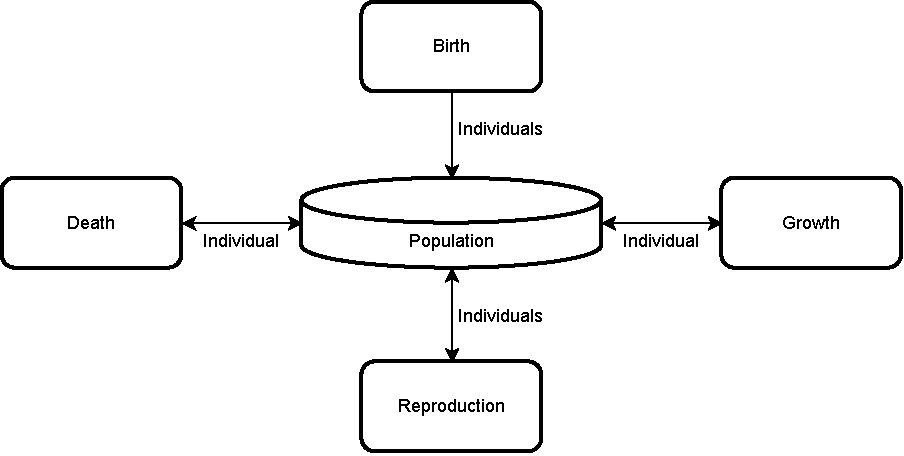
\includegraphics[width=80mm]{img/fig_algorithm_model.pdf}
    \caption{Animal Life Cycle Algorithm model.} \label{fig.algorithm_model}
    \end{figure}

\subsection{Problem}

In this algorithm's reproduction process, we find mating couples by mutual
attraction, where sometimes individuals won't procreate offspring because of
the mate's low appeal. As time passes, the environment could kill its
individuals either because they have low fitness or age, leading to extinction,
meaning there are no more individuals in the population left to reproduce. When
this condition presents, if evaluations are available and termination
conditions enable the algorithm to continue the search, it is required to
create a new set of individuals. We illustrate the general flowchart for the
Life-Cycle algorithm in Figure~\ref{fig.flowchart}.

\begin{figure}
    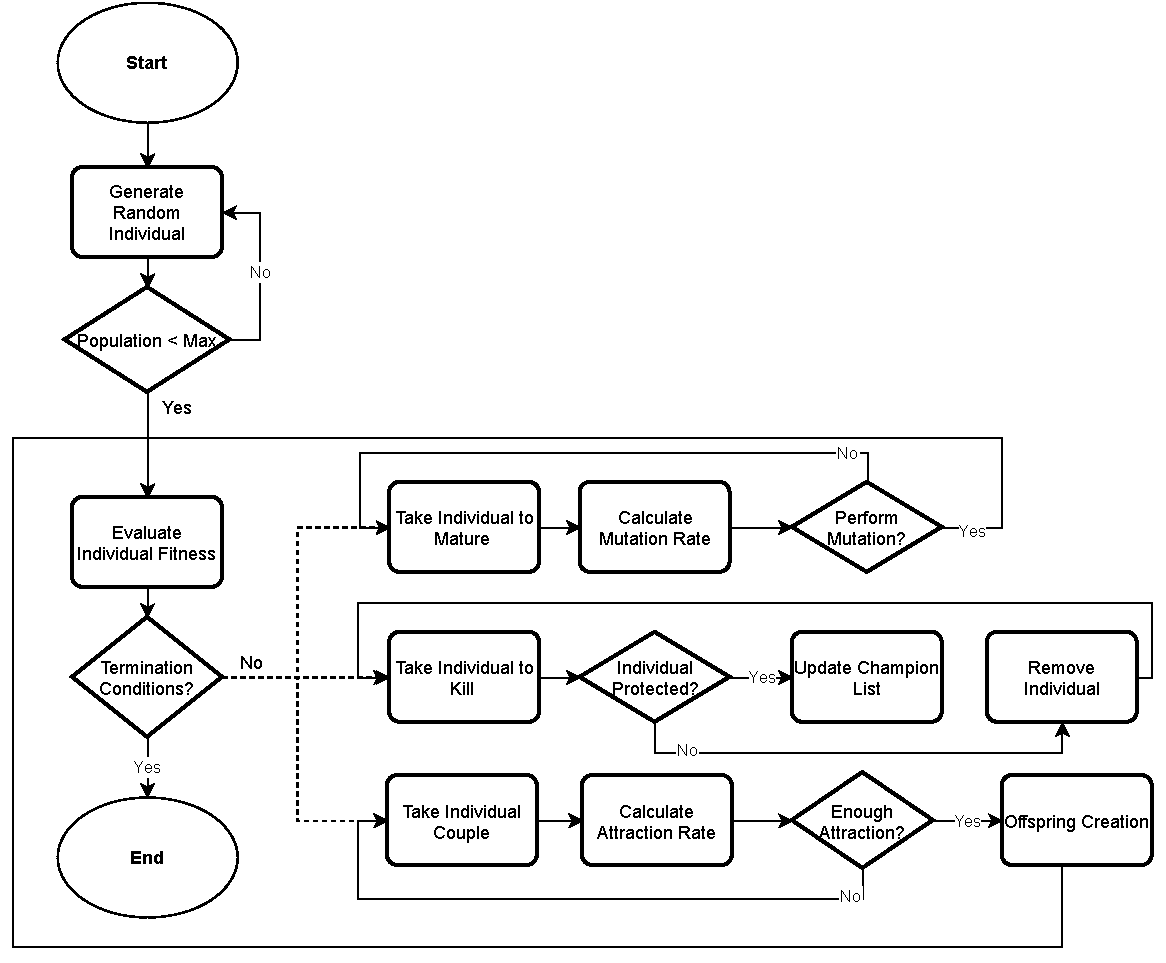
\includegraphics[width=\textwidth]{img/fig_flowchart.pdf}
    \caption{Animal Life-Cycle Algorithm general flowchart.} \label{fig.flowchart}
    \end{figure}

\subsection{Proposed Solution}

In this article, we test various strategies to generate a new population to
replace individuals that have already died (or were discarded) due to their
aptitude, as happens in the life cycle. We previously used to generate a new
random set of solutions, with the cost of losing all evolution knowledge. The
strategy we describe in this paper uses elites to take advantage of the
historical evolution, especially the best individuals, where we look for the
offspring of the elite set to be somewhat close to them. We use the golden
ratio to compute the distance between new individuals in the population, making
an improved distribution.

We propose one promising alternative to restart the population, to solve
extinction caused by nature's pressure in the Life Cycle algorithm: the
projection of the historically best-found candidate solutions (Elite) towards
the best-found candidate solution (Champion). This article proposes some
strategies to carry out this operation, where the presented distribution
strategy obtained the best results.

\subsubsection{How does it work?} Based on the historically best candidate
solution and the elite set, we use the Golden Ratio (shown in
Figure~\ref{fig.golden_ratio}) to compute the distance between new individuals
in the population, making an improved distribution. It randomly selects a
solution from the elite set and uses the Golden Ratio to compute multiple
solutions against the best-found candidate.

\begin{figure}
    \centering
    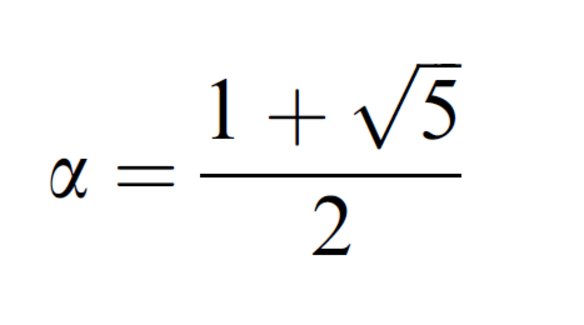
\includegraphics[width=25mm]{img/fig_golden_ratio.pdf}
    \caption{Golden Ratio equation.} \label{fig.golden_ratio}
    \end{figure}

This strategy is how we can calculate the projection of the historically
best-found candidate solutions (Elite) towards the best-found candidate
solution (Champion). To illustrate this concept we include
Figure~\ref{fig.elite_projection}, placing the Elite solution on the far right
and the Champion solution on the left corner, where a higher number of new
solutions will be closer to the Champion.

\begin{figure}
    \centering
    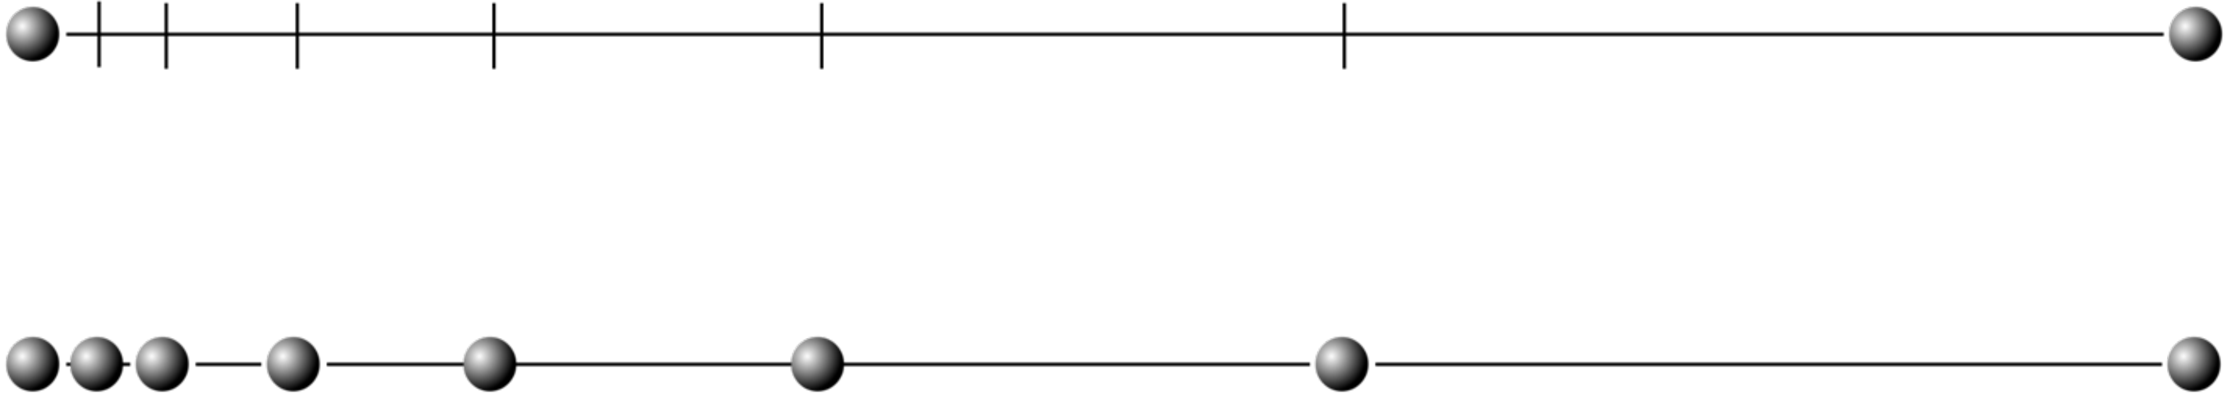
\includegraphics[width=0.65\textwidth]{img/fig_elite_projection.pdf}
    \caption{Projection of the historically Elite solutions towards the Champion.} \label{fig.elite_projection}
    \end{figure}

This process generates new solutions that will be the new population set. It
uses the Golden Ratio to progressively approximate from an Elite solution to
the Champion. This strategy facilitates to find apparently hidden solutions,
having an exploitation emphasis. Figure~\ref{fig.elite_projection_swarm}
displays the projection of five Elite solutions (on the corners) towards the
Champion (in the center).

\begin{figure}
    \centering
    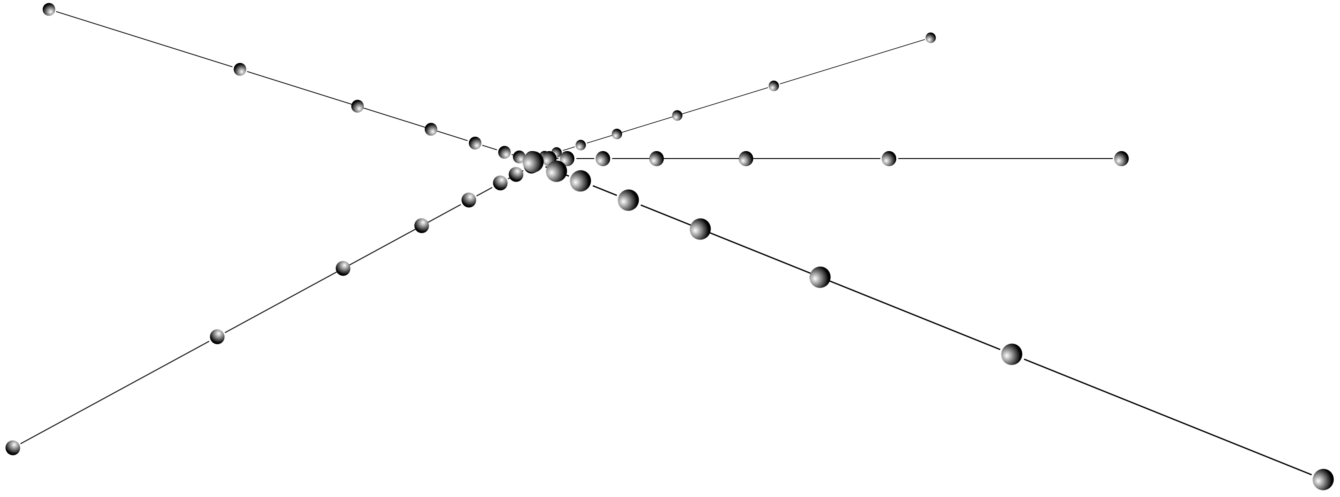
\includegraphics[width=0.85\textwidth]{img/fig_elite_projection_swarm.pdf}
    \caption{Projection of five Elite solutions towards the Champion, results in a mini-swarm.} \label{fig.elite_projection_swarm}
    \end{figure}

\section{Experiments}
\label{section.experiments}

As a proof-of-concept, we implemented the algorithm with Docker containers,
where we compare the results obtained with the projection of the Elite towards
the Champion strategy and the random use of the more traditional alternatives
(such as mutation and crossover), using classic benchmark functions for
optimization as implemented by the DEAP (Distributed Evolutionary Algorithms in
Python) library \cite{fortin2012deap}.

\subsection{Experimental Setup} 

The following tables show the configuration used to execute the experiments for
the analysis and comparison in this paper. In
Table~\ref{tab.general_configuration}, we can find the General Configuration
for the Animal Life Cycle Algorithm. All values from this configuration
remained constant during all phases of the experiment runs. The following
table, Table~\ref{tab.benchmark_fun_config}, shows the values used for the
Classic Benchmark Functions for Optimization, where these are adjusted
accordingly for each function.

% Please add the following required packages to your document preamble:
% \usepackage{booktabs}
% To change the size of the font use \scriptsize or \tiny
\begin{table}[]
    \scriptsize
    \centering
    \caption{Animal Life Cycle Algorithm (ALCA) General Configuration.}\label{tab.general_configuration}
    \begin{tabular}{@{}ll@{}}
    \toprule
    \multicolumn{2}{l}{\textbf{ALCA General Configuration}} \\ \midrule
    Function name & ALL \\
    Population & 500 \\
    Target error & 1.00E-08 \\
    Crossover rate & 100 \\
    Mutation rate & 7 \\
    Max age & 40 \\
    Tournament rep. & 100 \\
    Sample size & 20 \\
    Base approval & 80 \\
    Goal approval & 200 \\ \bottomrule
    \end{tabular}
    \end{table}

\begin{table}[]
    \scriptsize
    \centering
    \caption{Classic Benchmark Functions for Optimization Configuration.}\label{tab.benchmark_fun_config}
    \begin{tabular}{@{}llllllll@{}}
    \toprule
    \multicolumn{8}{l}{\textbf{Benchmark Configuration Setup}} \\ \midrule
    Function name & Ackley & Bohachevsky & Griewank & Rastrigin & Sphere & Rosenbrock & Rosenbrock \\
    Dimensions & 5, 10 & 5, 10 & 5, 10 & 5, 10 & 5, 10 & 5 & 10 \\
    Max evaluations & 200,000 & 200,000 & 200,000 & 200,000 & 200,000 & 500,000 & 1,000,000 \\
    Max stagnation & 50,000 & 50,000 & 50,000 & 50,000 & 50,000 & 125,000 & 250,000 \\
    Target fitness & -20.0 & -12.0 & -150.0 & -80.0 & -50.0 & -3500.0 & -3500.0 \\
    Bound matrix & {[}-32, 32{]} & {[}-2, 2{]} & {[}-500, 500{]} & {[}-5, 5{]} & {[}-5, 5{]} & {[}-2, 2{]} & {[}-2, 2{]} \\ \bottomrule
    \end{tabular}
    \end{table}


\subsection{Experiment Results}

For each experiment, we ran 30 independent executions per algorithm and
dimensions specified. We recorded the following results: best found error,
standard deviation, total number of evaluations, and total elapsed time (in
seconds). The labels used on the results of our summarized experiments tables
are the following:

\begin{itemize}
    \item   Error:       is the best found error (or best solution).
    \item   St-Dev:      is the standard deviation calculated from the error. 
    \item   Evals.:      is the total number of evaluations the algorithm executed.
    \item   Time:        is the total elapsed or wall clock time, in seconds. 
\end{itemize}

The alternatives to restart this new population are the creation of a new set
of candidate solutions based on either: 1. Crossing the Champion with the Elite;
2. The mutation with uniform modification from the Elite; 3. The
projection of the Elite towards the Champion; 4. Based on random use of the
previous alternatives. We compared three strategies by grouping the previous
alternatives in the following:

\begin{itemize}
    \item   Xover Mutation:      Crossing the Champion with the Elite, and the mutation with uniform modification from the Elite.
    \item   Elite Projection:    The projection of the Elite towards the Champion. 
    \item   All Random:          Based on random use of the previous alternatives.
\end{itemize}

\subsubsection{Ackley Benchmark Function Experiment}

\begin{figure}
    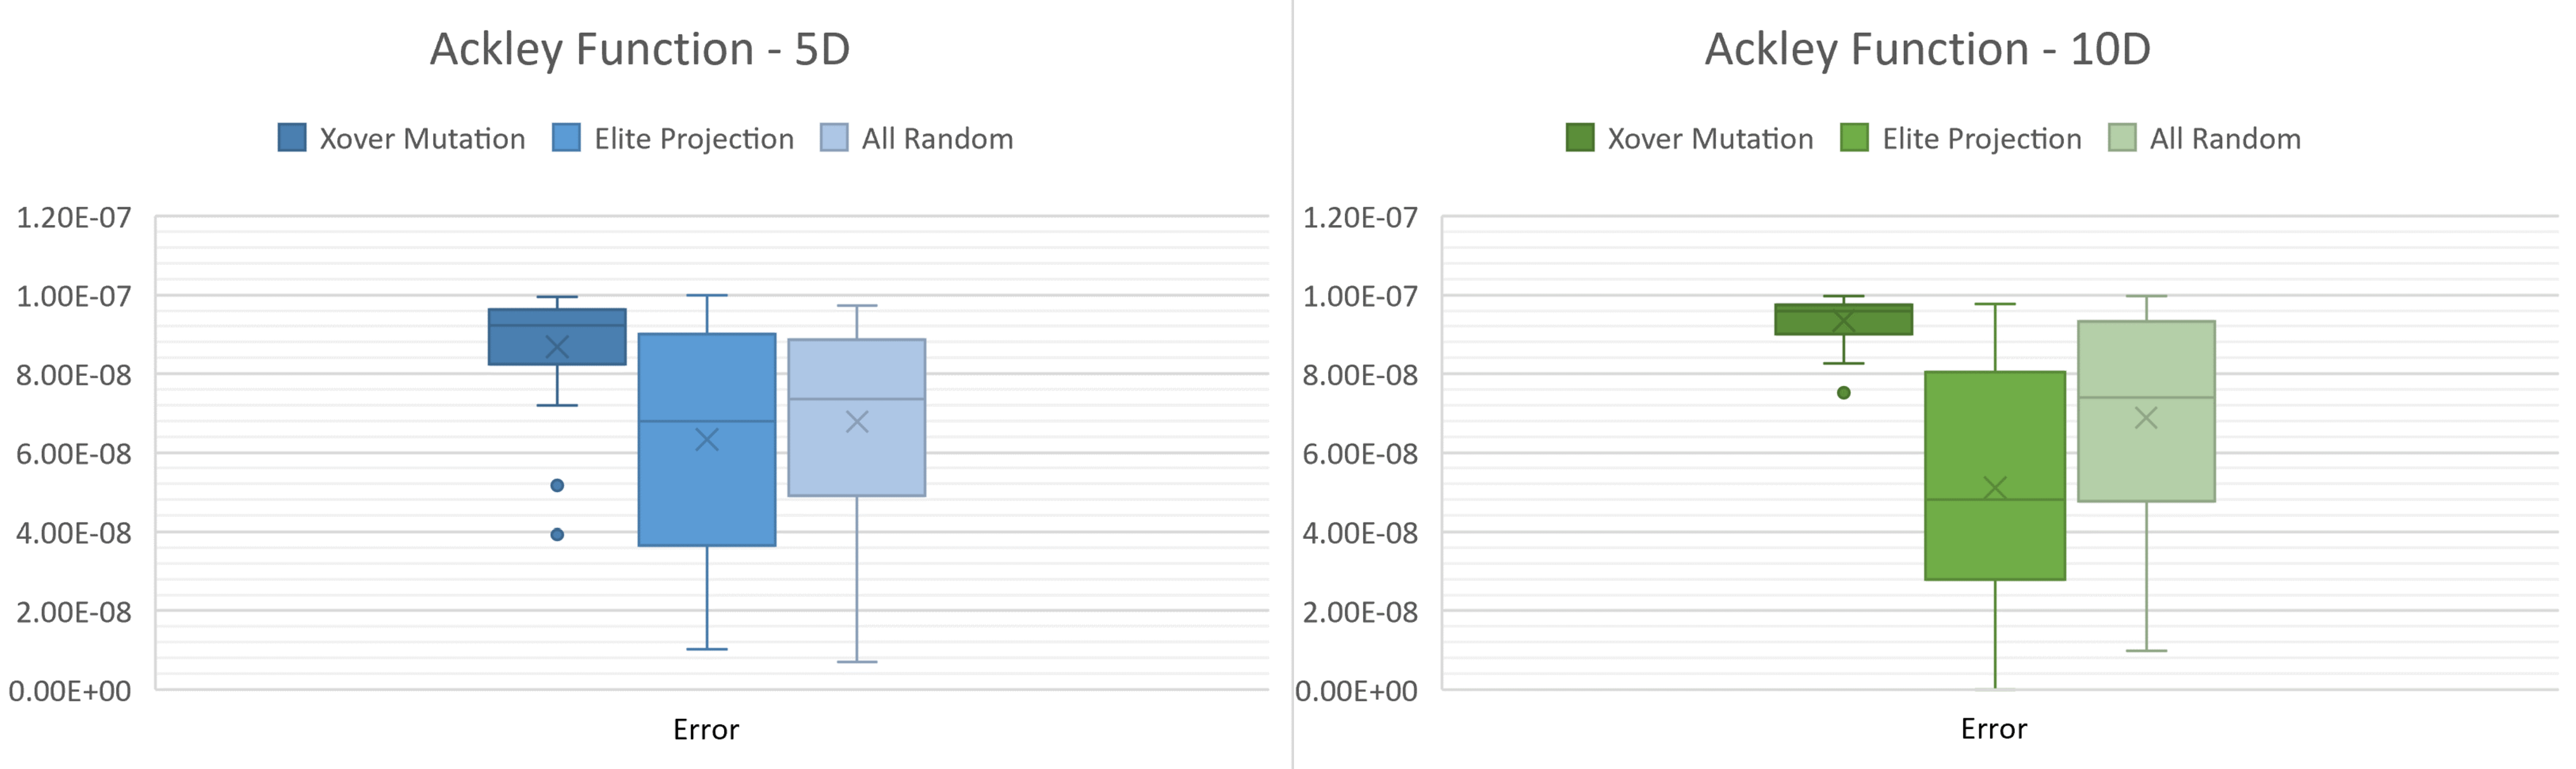
\includegraphics[width=\textwidth]{img/fig_fun_ackley.pdf}
    \caption{Box and whisker chart for the Ackley Benchmark Function, 5 vs 10 Dimensions.} \label{fig.fun_ackley}
    \end{figure}

\begin{table}[]
    \scriptsize
    \centering
    \caption{Ackley Benchmark Function summarized experiments table for 5 Dimensions.}\label{tab.fun_ackley5}
    \begin{tabular}{@{}lllll@{}}
    \toprule
    \multicolumn{5}{l}{\textbf{Ackley Function - 5 Dimensions}} \\ \midrule
     & \textbf{Error} & \textbf{St-Dev} & \textbf{Evals.} & \textbf{Time} \\
    \textbf{Xover Mutation} & 8.69E-08 & 1.36E-08 & 46,331 & 49.9 \\
    \textbf{Elite Projection} & 6.33E-08 & 2.70E-08 & 13,811 & 18.1 \\
    \textbf{All Random} & 6.78E-08 & 2.55E-08 & 30,236 & 32.8 \\ \bottomrule
    \end{tabular}
    \end{table}

\begin{table}[]
    \scriptsize
    \centering
    \caption{Ackley Benchmark Function summarized experiments table for 10 Dimensions.}\label{tab.fun_ackley10}
    \begin{tabular}{@{}lllll@{}}
    \toprule
    \multicolumn{5}{l}{\textbf{Ackley Function - 10 Dimensions}} \\ \midrule
     & \textbf{Error} & \textbf{St-Dev} & \textbf{Evals.} & \textbf{Time} \\
    \textbf{Xover Mutation} & 9.35E-08 & 5.93E-09 & 104,842 & 111.7 \\
    \textbf{Elite Projection} & 5.11E-08 & 3.13E-08 & 16,019 & 20.1 \\
    \textbf{All Random} & 6.89E-08 & 2.75E-08 & 43,631 & 46.3 \\ \bottomrule
    \end{tabular}
    \end{table}


\subsubsection{Bohachevsky Benchmark Function Experiment}

\begin{figure}
    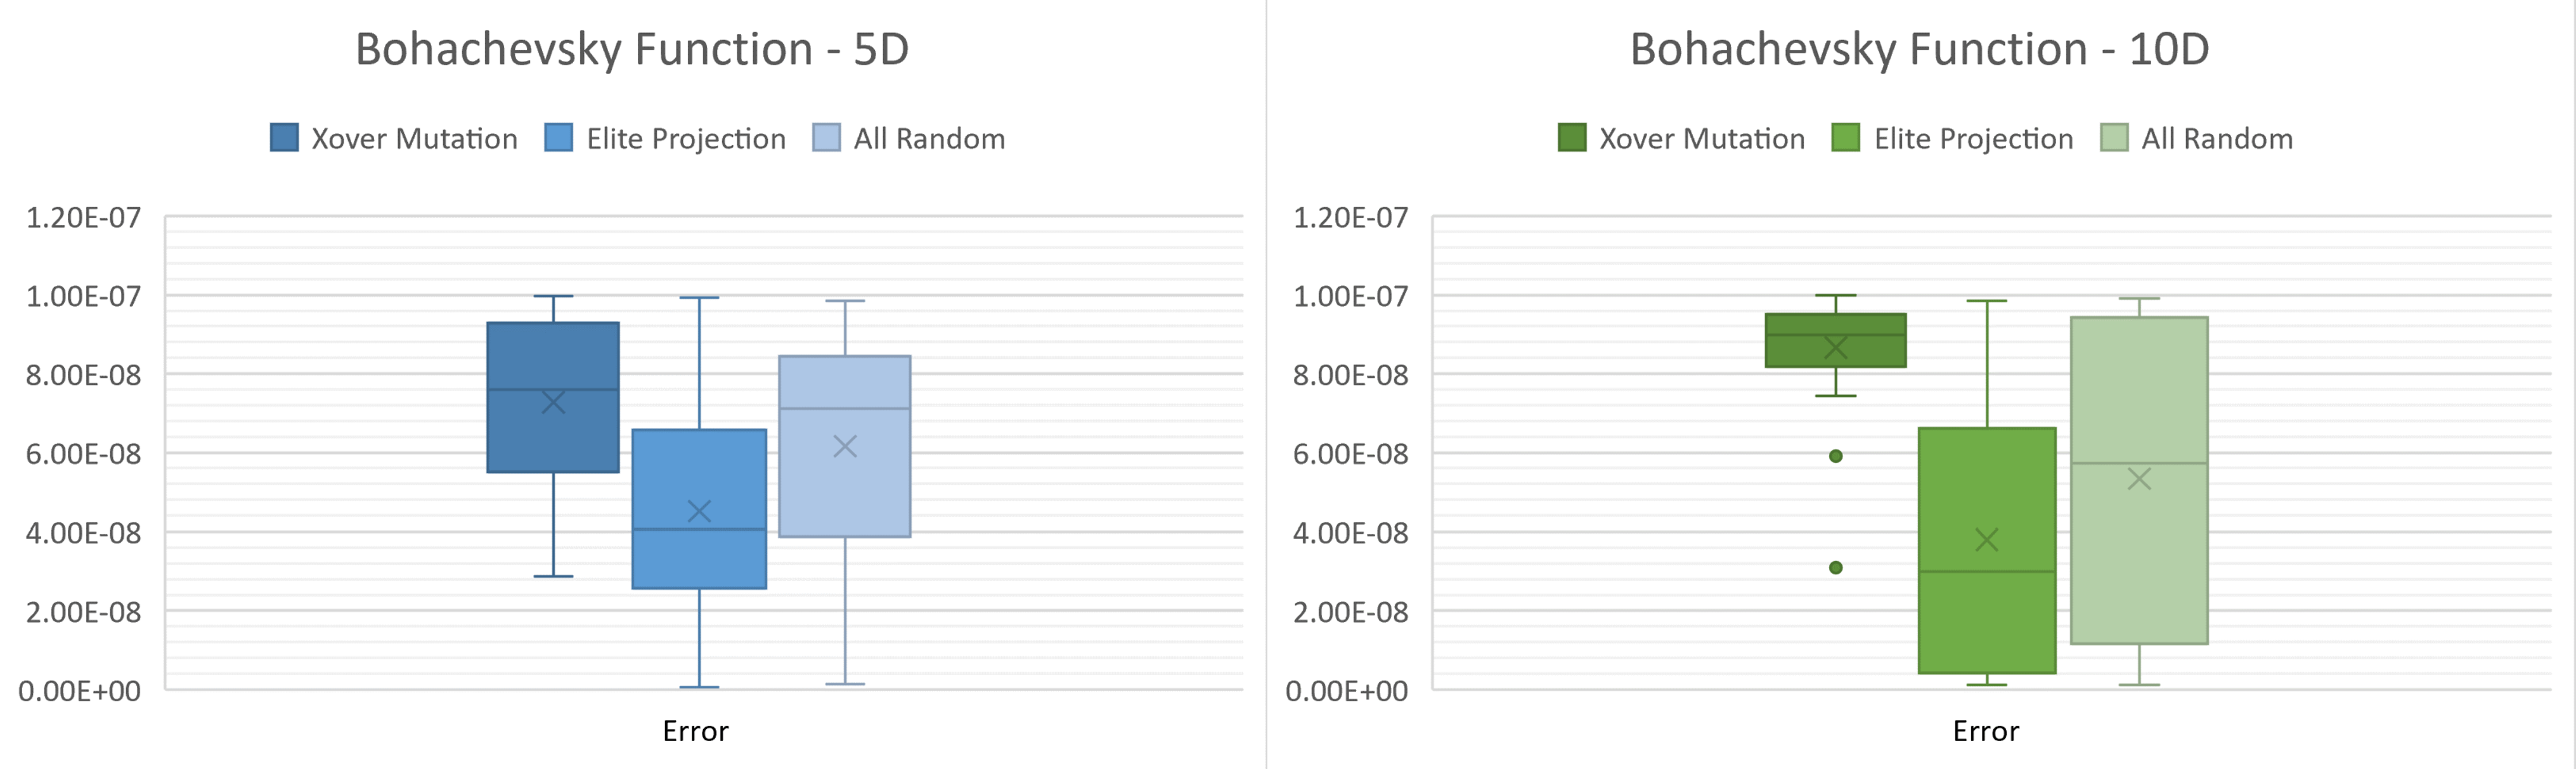
\includegraphics[width=\textwidth]{img/fig_fun_bohachevsky.pdf}
    \caption{Box and whisker chart for the Bohachevsky Benchmark Function, 5 vs 10 Dimensions.} \label{fig.fun_bohachevsky}
    \end{figure}

\begin{table}[]
    \scriptsize
    \centering
    \caption{Bohachevsky Benchmark Function summarized experiments table for 5 Dimensions.}\label{tab.fun_bohachevsky5}
    \begin{tabular}{@{}lllll@{}}
    \toprule
    \multicolumn{5}{l}{\textbf{Bohachevsky Function - 5 Dimensions}} \\ \midrule
     & \textbf{Error} & \textbf{St-Dev} & \textbf{Evals.} & \textbf{Time} \\
    \textbf{Xover Mutation} & 7.28E-08 & 2.20E-08 & 15,010 & 24.2 \\
    \textbf{Elite Projection} & 4.51E-08 & 2.94E-08 & 8,266 & 12.6 \\
    \textbf{All Random} & 6.16E-08 & 2.85E-08 & 11,998 & 21.7 \\ \bottomrule
    \end{tabular}
    \end{table}

\begin{table}[]
    \scriptsize
    \centering
    \caption{Bohachevsky Benchmark Function summarized experiments table for 10 Dimensions.}\label{tab.fun_bohachevsky10}
    \begin{tabular}{@{}lllll@{}}
    \toprule
    \multicolumn{5}{l}{\textbf{Bohachevsky Function - 10 Dimensions}} \\ \midrule
     & \textbf{Error} & \textbf{St-Dev} & \textbf{Evals.} & \textbf{Time} \\
    \textbf{Xover Mutation} & 8.66E-08 & 1.38E-08 & 40,166 & 44.4 \\
    \textbf{Elite Projection} & 3.80E-08 & 3.34E-08 & 8,506 & 12.9 \\
    \textbf{All Random} & 5.34E-08 & 3.76E-08 & 19,537 & 26.8 \\ \bottomrule
    \end{tabular}
    \end{table}


\subsubsection{Griewank Benchmark Function Experiment}

\begin{figure}
    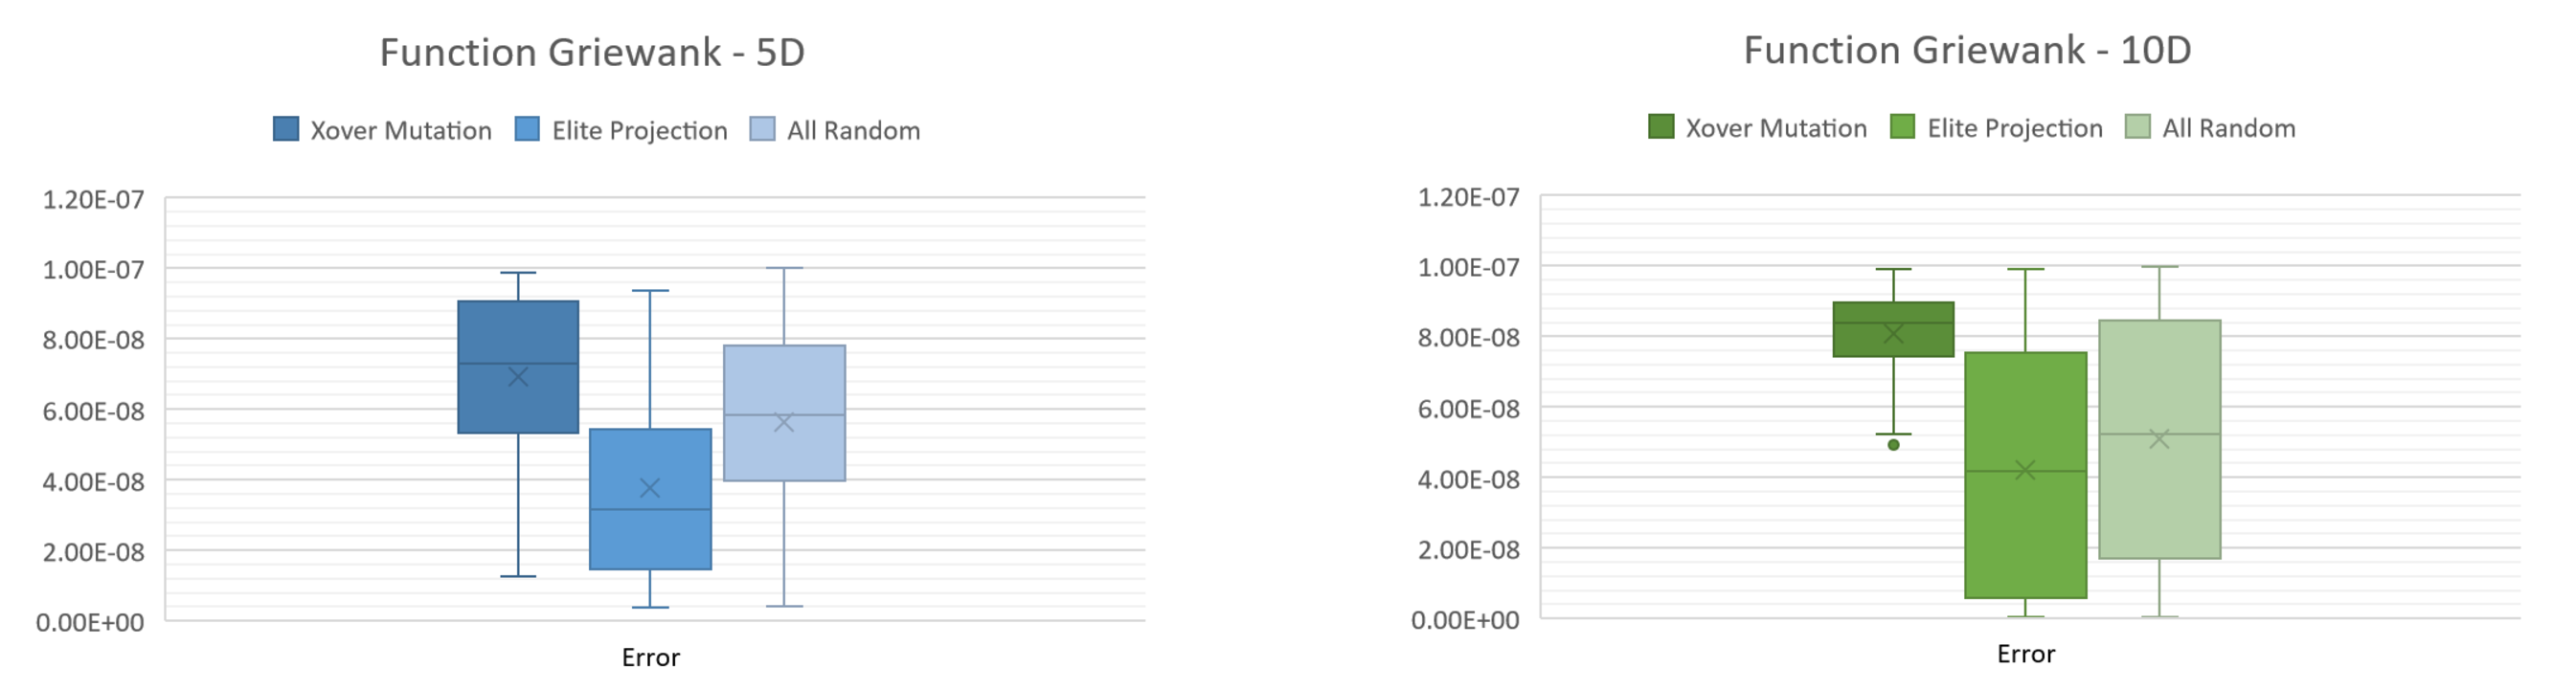
\includegraphics[width=\textwidth]{img/fig_fun_griewank.pdf}
    \caption{Box and whisker chart for the Griewank Benchmark Function, 5 vs 10 Dimensions.} \label{fig.fun_griewank}
    \end{figure}

\begin{table}[]
    \scriptsize
    \centering
    \caption{Griewank Benchmark Function summarized experiments table for 5 Dimensions.}\label{tab.fun_griewank5}
    \begin{tabular}{@{}lllll@{}}
    \toprule
    \multicolumn{5}{l}{\textbf{Griewank Function - 5 Dimensions}} \\ \midrule
     & \textbf{Error} & \textbf{St-Dev} & \textbf{Evals.} & \textbf{Time} \\
    \textbf{Xover Mutation} & 6.92E-08 & 2.40E-08 & 44,566 & 48.3 \\
    \textbf{Elite Projection} & 3.77E-08 & 2.74E-08 & 16,412 & 20.1 \\
    \textbf{All Random} & 5.63E-08 & 2.99E-08 & 35,761 & 38.5 \\ \bottomrule
    \end{tabular}
    \end{table}

\begin{table}[]
    \scriptsize
    \centering
    \caption{Griewank Benchmark Function summarized experiments table for 10 Dimensions.}\label{tab.fun_griewank10}
    \begin{tabular}{@{}lllll@{}}
    \toprule
    \multicolumn{5}{l}{\textbf{Griewank Function - 10 Dimensions}} \\ \midrule
     & \textbf{Error} & \textbf{St-Dev} & \textbf{Evals.} & \textbf{Time} \\
    \textbf{Xover Mutation} & 8.07E-08 & 1.39E-08 & 92,885 & 100.0 \\
    \textbf{Elite Projection} & 4.21E-08 & 3.40E-08 & 13,534 & 17.3 \\
    \textbf{All Random} & 5.08E-08 & 3.54E-08 & 40,544 & 52.5 \\ \bottomrule
    \end{tabular}
    \end{table}


\subsubsection{Rastrigin Benchmark Function Experiment}

\begin{figure}
    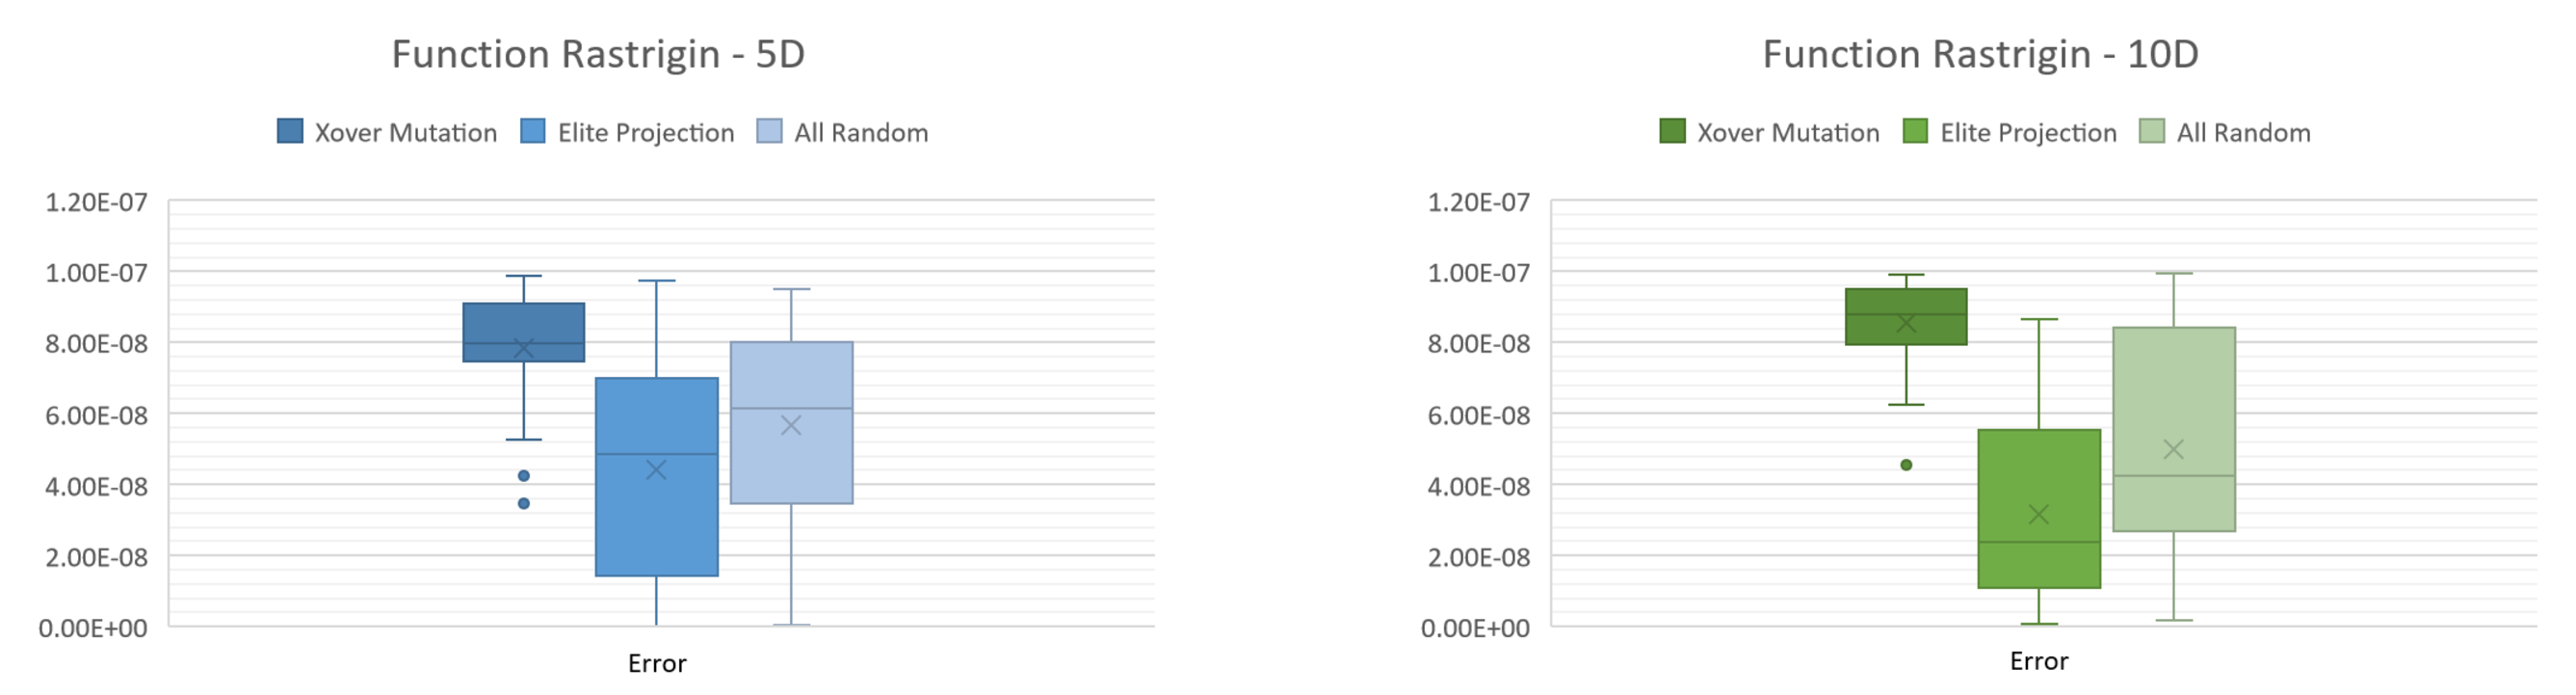
\includegraphics[width=\textwidth]{img/fig_fun_rastrigin.pdf}
    \caption{Box and whisker chart for the Rastrigin Benchmark Function, 5 vs 10 Dimensions.} \label{fig.fun_rastrigin}
    \end{figure}

\begin{table}[]
    \scriptsize
    \centering
    \caption{Rastrigin Benchmark Function summarized experiments table for 5 Dimensions.}\label{tab.fun_rastrigin5}
    \begin{tabular}{@{}lllll@{}}
    \toprule
    \multicolumn{5}{l}{\textbf{Rastrigin Function - 5 Dimensions}} \\ \midrule
     & \textbf{Error} & \textbf{St-Dev} & \textbf{Evals.} & \textbf{Time} \\
    \textbf{Xover Mutation} & 7.85E-08 & 1.59E-08 & 22,322 & 34.1 \\
    \textbf{Elite Projection} & 4.42E-08 & 3.26E-08 & 10,860 & 14.8 \\
    \textbf{All Random} & 5.66E-08 & 2.81E-08 & 21,122 & 35.0 \\ \bottomrule
    \end{tabular}
    \end{table}

\begin{table}[]
    \scriptsize
    \centering
    \caption{Rastrigin Benchmark Function summarized experiments table for 10 Dimensions.}\label{tab.fun_rastrigin10}
    \begin{tabular}{@{}lllll@{}}
    \toprule
    \multicolumn{5}{l}{\textbf{Rastrigin Function - 10   Dimensions}} \\ \midrule
     & \textbf{Error} & \textbf{St-Dev} & \textbf{Evals.} & \textbf{Time} \\
    \textbf{Xover Mutation} & 8.56E-08 & 1.23E-08 & 53,579 & 58.7 \\
    \textbf{Elite Projection} & 3.17E-08 & 2.57E-08 & 8,704 & 13.0 \\
    \textbf{All Random} & 5.00E-08 & 3.16E-08 & 24,376 & 27.4 \\ \bottomrule
    \end{tabular}
    \end{table}


\subsubsection{Sphere Benchmark Function Experiment}

\begin{figure}
    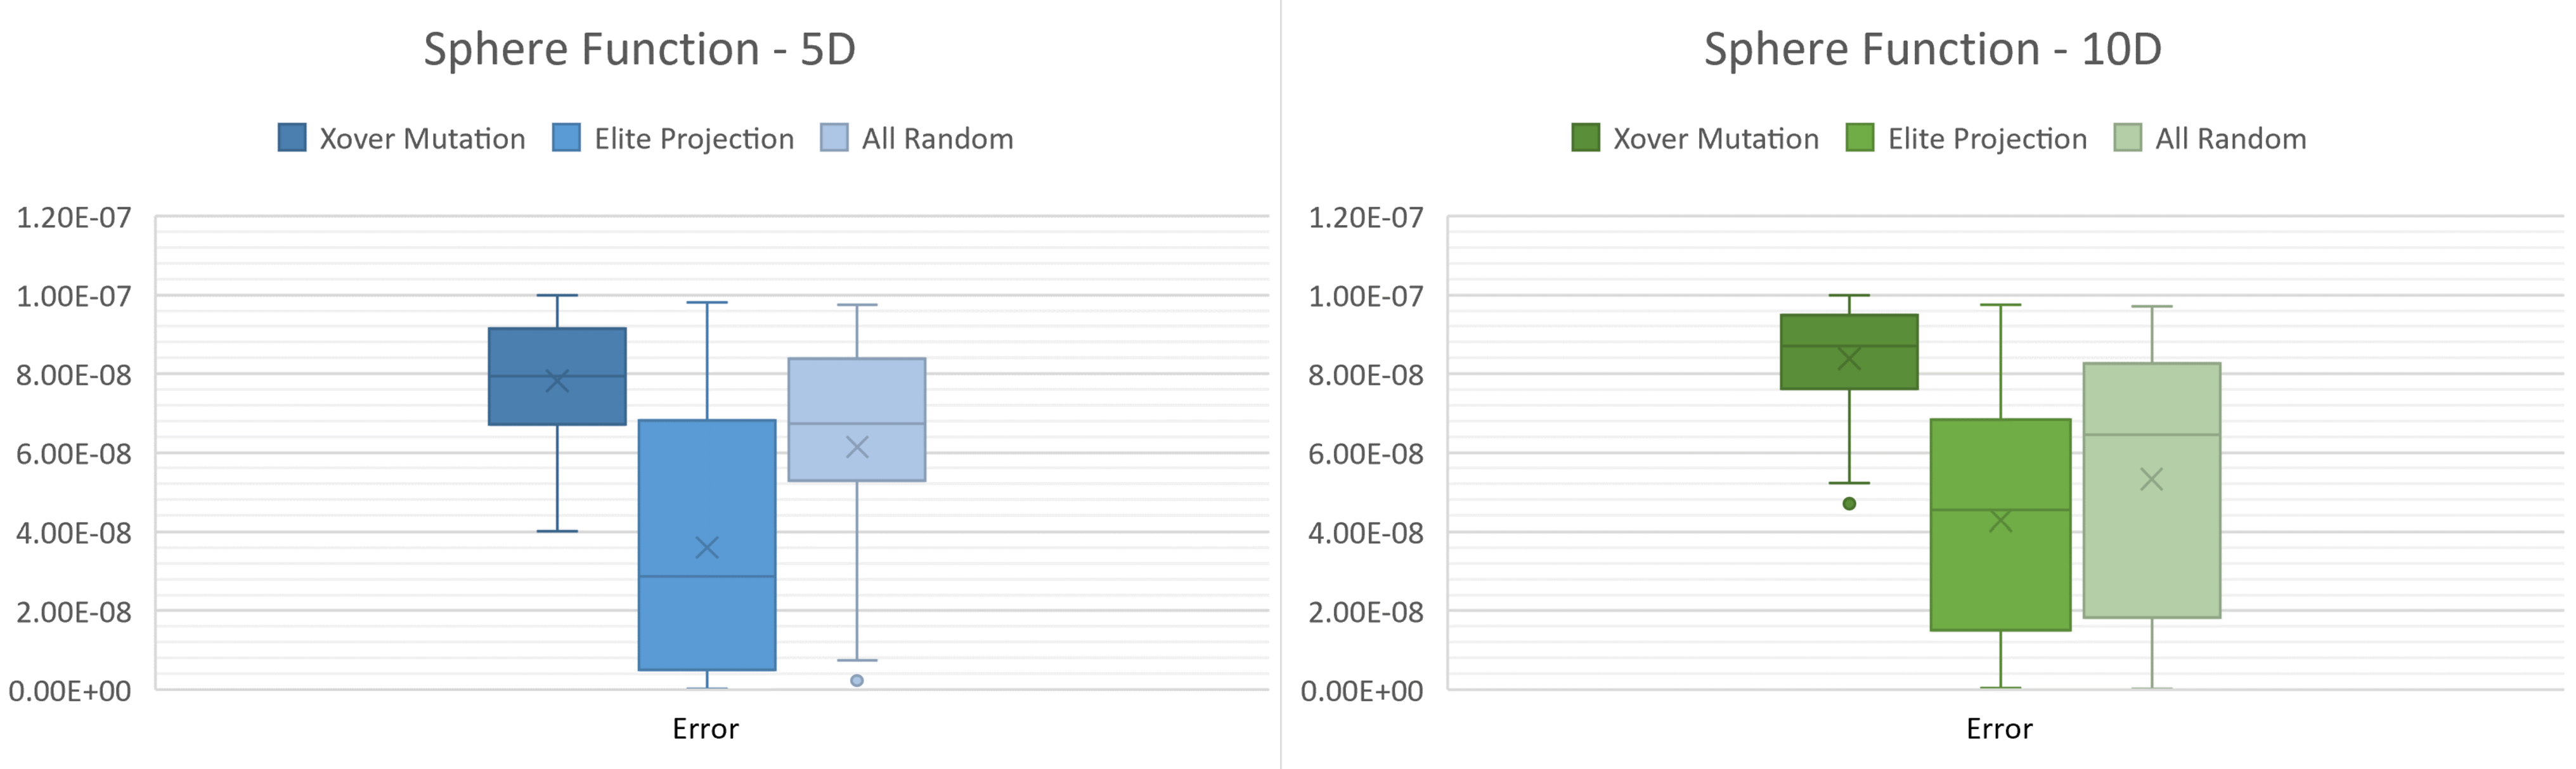
\includegraphics[width=\textwidth]{img/fig_fun_sphere.pdf}
    \caption{Box and whisker chart for the Sphere Benchmark Function, 5 vs 10 Dimensions.} \label{fig.fun_sphere}
    \end{figure}

\begin{table}[]
    \scriptsize
    \centering
    \caption{Sphere Benchmark Function summarized experiments table for 5 Dimensions.}\label{tab.fun_sphere5}
    \begin{tabular}{@{}lllll@{}}
    \toprule
    \multicolumn{5}{l}{\textbf{Sphere Function - 5 Dimensions}} \\ \midrule
     & \textbf{Error} & \textbf{St-Dev} & \textbf{Evals.} & \textbf{Time} \\
    \textbf{Xover Mutation} & 7.82E-08 & 1.65E-08 & 11,312 & 14.5 \\
    \textbf{Elite Projection} & 3.60E-08 & 3.27E-08 & 7,056 & 10.9 \\
    \textbf{All Random} & 6.14E-08 & 2.79E-08 & 9,158 & 12.2 \\ \bottomrule
    \end{tabular}
    \end{table}

\begin{table}[]
    \scriptsize
    \centering
    \caption{Sphere Benchmark Function summarized experiments table for 10 Dimensions.}\label{tab.fun_sphere10}
    \begin{tabular}{@{}lllll@{}}
    \toprule
    \multicolumn{5}{l}{\textbf{Sphere Function - 10 Dimensions}} \\ \midrule
     & \textbf{Error} & \textbf{St-Dev} & \textbf{Evals.} & \textbf{Time} \\
    \textbf{Xover Mutation} & 8.39E-08 & 1.45E-08 & 30,769 & 34.4 \\
    \textbf{Elite Projection} & 4.28E-08 & 3.06E-08 & 9,236 & 13.3 \\
    \textbf{All Random} & 5.32E-08 & 3.38E-08 & 21,465 & 26.3 \\ \bottomrule
    \end{tabular}
    \end{table}

\subsection{ALTO / HASTA AQUI VAMOS}

\section{Discussion}
\label{section.discussion}

At some crucial moments during our research, we got the feeling we were doing
nature reverse engineering. One strategy was to let our imagination run wild
and go for the simple solution. One of our earlier experiment's findings was to
find balance, like the yin and yang, between death and reproduction.

In our experiments, we found that when solving simple problems, the cost of
communication between containers can become a factor to increase the total
performance time, even though, we believe that the opposite must also be true.
When solving complex problems, distributing the work on multiple resources
should reduce throughput time, making the communication cost negligible.

We must acknowledge the performance time of the DEAP library
\cite{fortin2012deap} is highly efficient and short, due in part because the
processing work execution is on a single processor with multiple cores, where
the communication time is nearly non-existent. In contrast, our algorithm
implementation requires a minimum of five containers and a message queue
server. Even though the container work has proven to be very effective and
efficient \cite{merelo2016performance,valdez2021container}, we must consider
some time was added to our experiments by the minimal delays (in the thousands
of a second magnitude) we used to keep the process execution relatively random,
to mimic how the life-cycle stages work in nature \cite{read1968system}. As
future work, we could test the Life-Cycle algorithm behavior by eliminating all
remaining delays.

This scheme allows for multiple parameter's fine tuning, granting us the
freedom to experiment with different selection and reproduction strategies
simultaneously, which will impact how fast it finds the solution and the
obtained quality.


\section{Conclusions}
\label{section.conclusions}

We implemented the algorithm with Docker containers by solving the OneMax
problem comparing it with a traditional (sequential) GA algorithm, where it
showed favorable and promising results. To further validate this work, we could
use control or some more complex and demanding problem that requires computing
real numbers \cite{stanley2002evolving,miikkulainen2019evolving}.

As the complexity of problems increases, it is essential to have a scalable,
replicable, and fault-tolerant model that uses collaborative techniques to work
in the cloud, where multiple resources will be communicating asynchronously.
This research has shown that it is possible to evolve a population of
individuals, similar to a Genetic Algorithm (GA), using a distributed,
parallel, and asynchronous methodology.

%----------------------------------------------------
%----------------------------------------------------
%PREVIOUSLY / FROM THE FIRST CHAPTER
%We designed our algorithm using observation, analysis, and abstraction in nature to identify what most species in the animal kingdom have in common, where individuals of a population that best adapt to the environment have greater chances of survival, reproduction, and improvement of the species. Imagining as if the task of writing these rules of evolution was in our hands, questioning how we could solve it?
%Like nature, we identified what most species have in common in the life cycle. Our algorithm works on a constantly evolving population, experiencing the stages that all living beings undergo \cite{read1968system}: being born, growing up, reproducing, and dying, where each of these stages will be processes (of our algorithm) that randomly affect the population individuals, emulating the organic way.
%Many of the publications with the most influence on our research ~\cite{valdez2021container,garcia2021event,merelo2016performance,merelo2016nodio} propose a cloud-native optimization architecture that features population-based algorithms. They present ideas such as those mentioned in Figure~\ref{fig.background}, which planted the seed of thought of our current paper.
%Some questions in our train of thought were: How does nature work? Is evolution real? How do we enforce natural selection in evolution? What is the role of the attraction between couples on reproduction? How much of a factor is the attraction's role in the evolution of the species? What is the role of death in all of this? How much of an impact does death have on the evolution of a species? How do we include those ideas into our algorithm?
%One of the main challenges when designing the algorithm was how to capture the essence of life by reflecting a population evolution?. In our minds, it was clear this task requires a combination of simultaneous working forces that influences the population improvement over time. Our strategy was simple: divide and conquer, looking into the clouds. Enter cloud-computing: previous cloud-computing algorithms have proven successful results working in optimization problems \cite{valdez2021container,garcia2021event}.
%We turned back to our genetic algorithms knowledge, mixed with our inspiration and cloud computing, and designed the algorithm with the quest to divide the processing workload among multiple computers. This strategy would also make it possible to run our algorithm as a cloud service. Theoretically, one consequence of the workload distribution is to obtain lower execution times.
%----------------------------------------------------
%Birth: This algorithm starts with a randomly generated population, where the processes will interact with the population independently. This means that at any given time, any individual can experience any of these processes. Birth is the first process of our algorithm, and it is responsible for the initial generation of individuals.
%Growth: As in nature, all individuals constantly grow, mature, or age. With increasing age, individuals may lose strength but also gain more knowledge to solve problems. We represent this with a possible mutation in each increment of age. The growth process will take an individual to assess whether it's ready to mature and undergo changes. 
%Reproduction: The attraction of a couple will depend on fitness: the better individual's fitness, the more attractive it will be, making it easier to find mating matches. This process will be taking random pairs of individuals to evaluate their attraction as a couple, to try to breed; when the gestation is successful, a new pair of individuals will be born (as the offspring). Not all couples will be compatible, so reproduction will not always be possible, but the problem arises: how to quantify the attraction between two individuals?
%------------- We could have used several strategies to evaluate this attraction. Considering this algorithm takes a similar focus as the study of bacteria growth in microbiology, where we can observe and analyze the evolution of a population over time. As in nature' most species, the bigger a specimen is, the more attractive it is to its mating candidates. To be consistent with both ideas in our algorithm, we use the equation of Newton's Law of Universal Gravitation (1) to calculate the attraction between two individuals, where we visualize the individual fitness as its mass when using the equation. In previous work, Newton's Law of Universal Gravitation has shown success in helping to solve optimization problems \cite{sanchez2014fuzzy,rashedi2009gsa}.
%Death: The death stage represents the challenges and adversities that life presents to overcome. This process evaluates the individual resistance to survive in the environment. The better fitness the individual has will increase its chances of survival. As time progresses, the demands of nature will also increase, pushing for only the best individuals to survive.
%----------------------------------------------------
%One strategic difference in our algorithm implementation is the reproduction process, which is flexible to work in parallel with multiple couple selection methods, for example, tournament selection, random selection (Closed Reproduction process), and couple match by creating a new mating individual (Open Reproduction process). We use many combinations of the containerized processes, up to the minimum number required to obtain good results. Figure~\ref{fig.processes_containers} shows a comparison of only two alternatives for the implementation of the algorithm. Our experimentation started with a configuration of ten processes and ended in five, shown on the left and right sides of Fig.~\ref{fig.processes_containers}, respectively.
%In our four experiments, we needed to match or balance the experimentation parameters according to the specifications of the algorithm used by the DEAP library. This is to be able to verify if our algorithm would also converge on the solutions in a similar number of evaluations and execution time. Table~\ref{tab.configuration} shows the OneMax initial configuration for DEAP and Life-Cycle experiment.
%----------------------------------------------------

\section{Another Section}
\label{section.another_section}

\subsection{Experiment Example}

\subsubsection{Experiment 1} The goal of our first OneMax experiment was to
make sure our Life-Cycle algorithm worked as expected, converging on the
solution. For this experiment, we intentionally used delays (on the tenth of a
second magnitude) to follow the Life-Cycle algorithm behavior on the console
output. For this experiment, we compared the DEAP algorithm versus the
Life-Cycle using ten processes (on containers) where we show the summarized
results in Table~\ref{tab.experiment1}, and Figure~\ref{fig.experiment1} shows
their Box and Whisker chart.

\begin{table}[]
    \centering        
    \caption{Experiment 1 results: OneMax DEAP versus Life-Cycle (10 processes).}\label{tab.experiment1}
    \begin{tabular}{|l|l|l|l|l|l|l|l|l|}
    \hline
    Run & \multicolumn{4}{l|}{OneMax DEAP} & \multicolumn{4}{l|}{Life-Cycle (10P)} \\ \hline
    1-60 & Last Gen. & Eval. & Time (sec) & Eval/sec & Last Gen. & Eval. & Time (sec) & Eval/sec \\ \hline
    Avg. & 6.5 & 391 & 0.036 & 10,836 & 9.6 & 578 & 6.830 & 85 \\ \hline
    \end{tabular}
    \end{table}

\begin{figure}
    \fbox{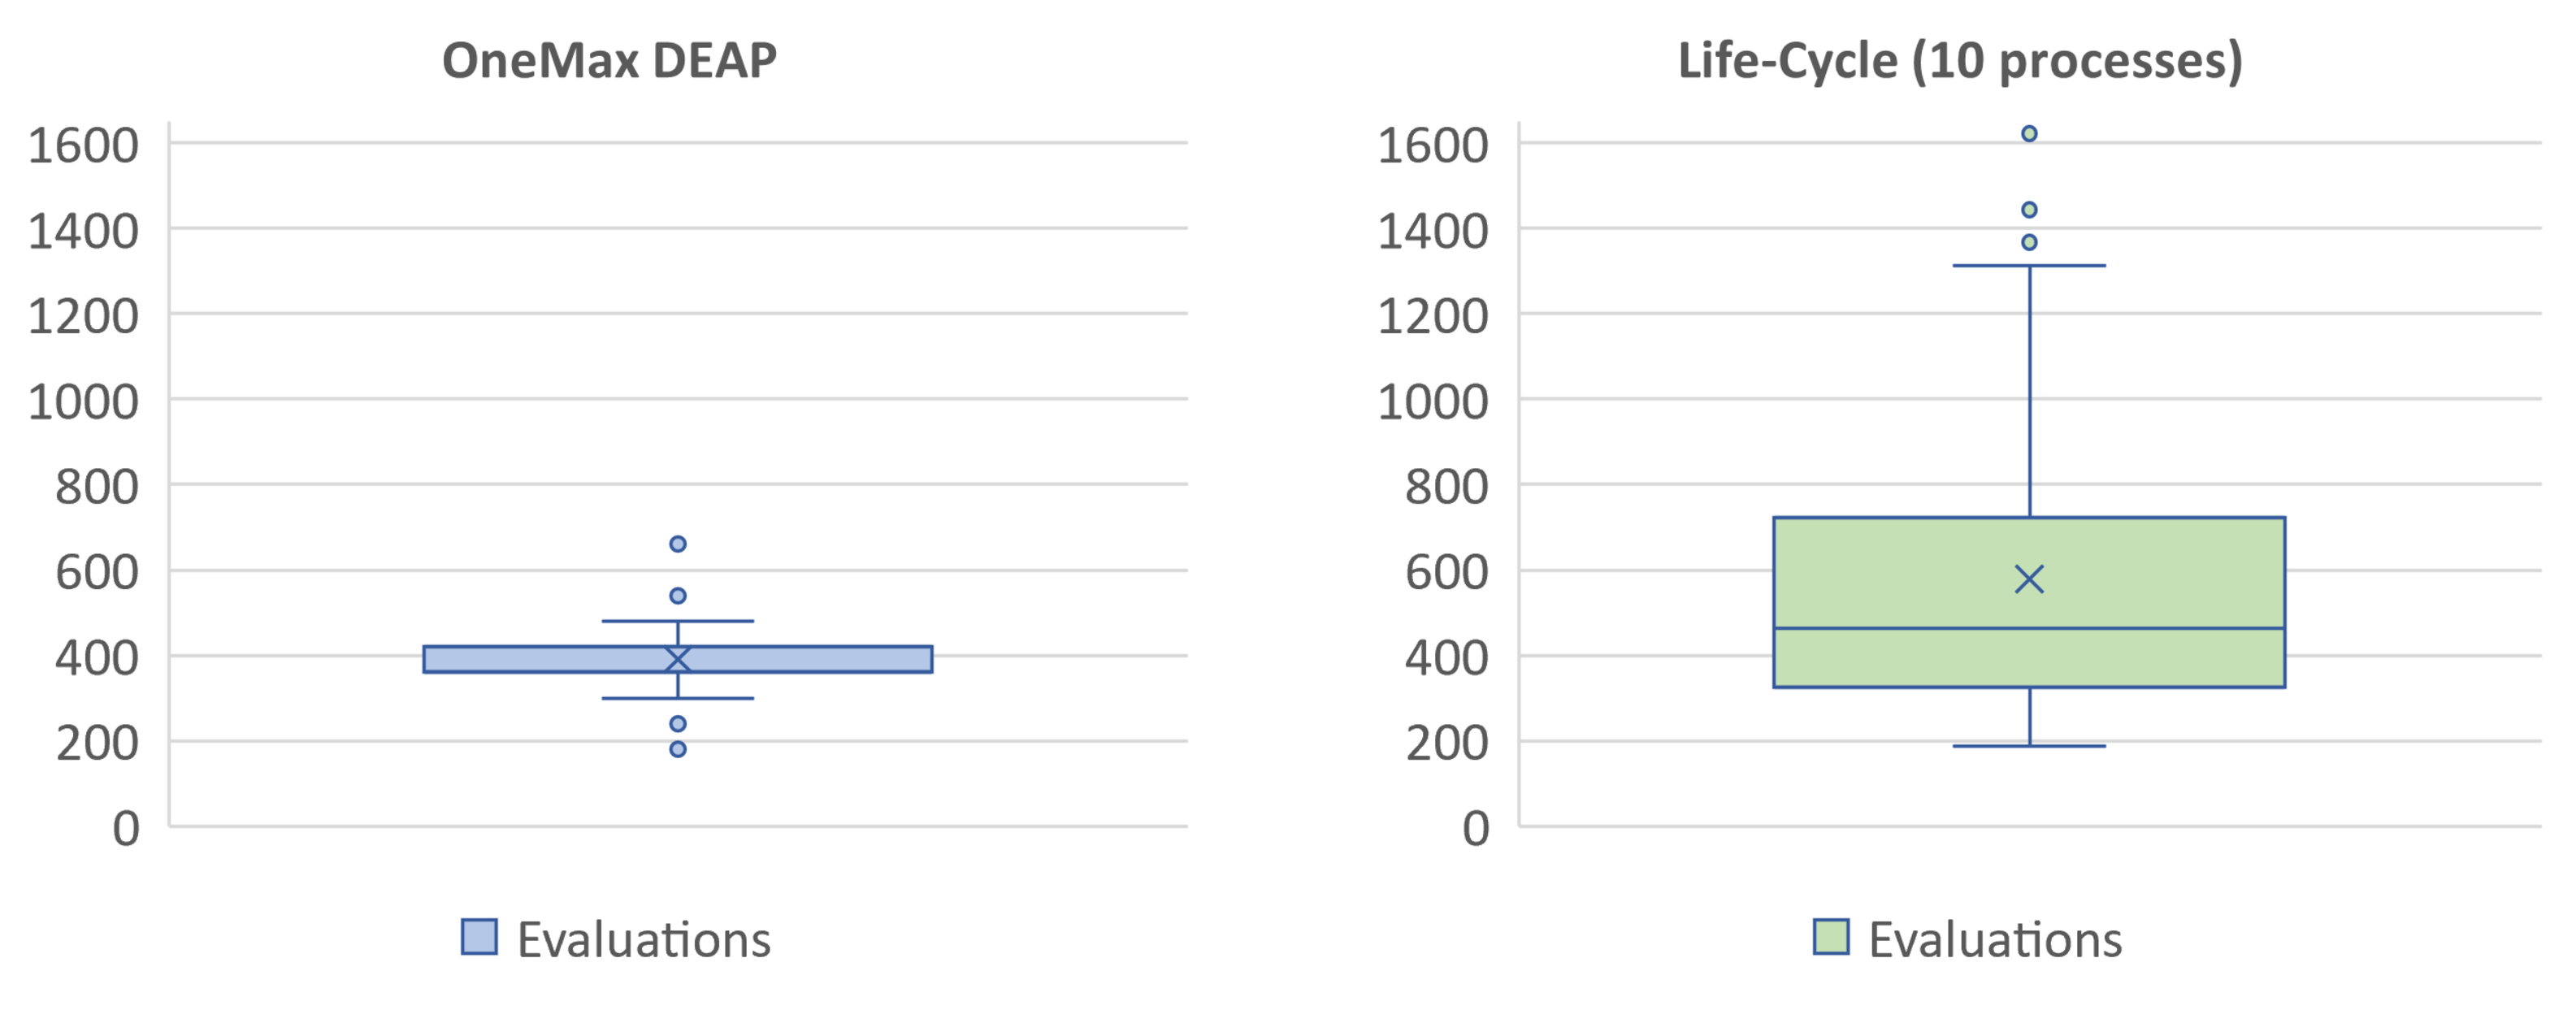
\includegraphics[width=\textwidth]{img/fig6_experiment01_chart.pdf}}
    \caption{Box and whisker chart for the Experiment 1: OneMax DEAP versus Life-Cycle.} \label{fig.experiment1}
% You need to label axis y - JJ
  \end{figure}


\subsubsection{Experiment 2} The goal of our second experiment was to confirm
the Life-Cycle algorithm continued working as expected, converging on the
solution. For this experiment, we reduced the time used on delays (now on the
thousands of a second magnitude) to follow the Life-Cycle algorithm behavior.
For this experiment, we only used tournament selection for the reproduction, on
the first configuration running the Life-Cycle on ten processes, versus the
second configuration where we reduced the processes to the minimum basic 5. We
show the summarized results in Table~\ref{tab.experiment2}, and
Figure~\ref{fig.experiment2} shows their Box and Whisker chart.

\begin{table}[]
    \centering        
    \caption{Experiment 2 results, Life-Cycle Tournament selection: 10 versus 5 processes.}\label{tab.experiment2}
    \begin{tabular}{|l|l|l|l|l|l|l|l|l|}
    \hline
    Run & \multicolumn{4}{l|}{LifeCycle (Tourn. 10P)} & \multicolumn{4}{l|}{LifeCycle (Tourn. 5P)} \\ \hline
    1-60 & Last Gen. & Eval. & Time (sec) & Eval/sec & Last Gen. & Eval. & Time (sec) & Eval/sec \\ \hline
    Avg. & 7.2 & 434 & 0.740 & 587 & 8.2 & 495 & 0.826 & 599 \\ \hline
    \end{tabular}
    \end{table}

\begin{figure}
    \fbox{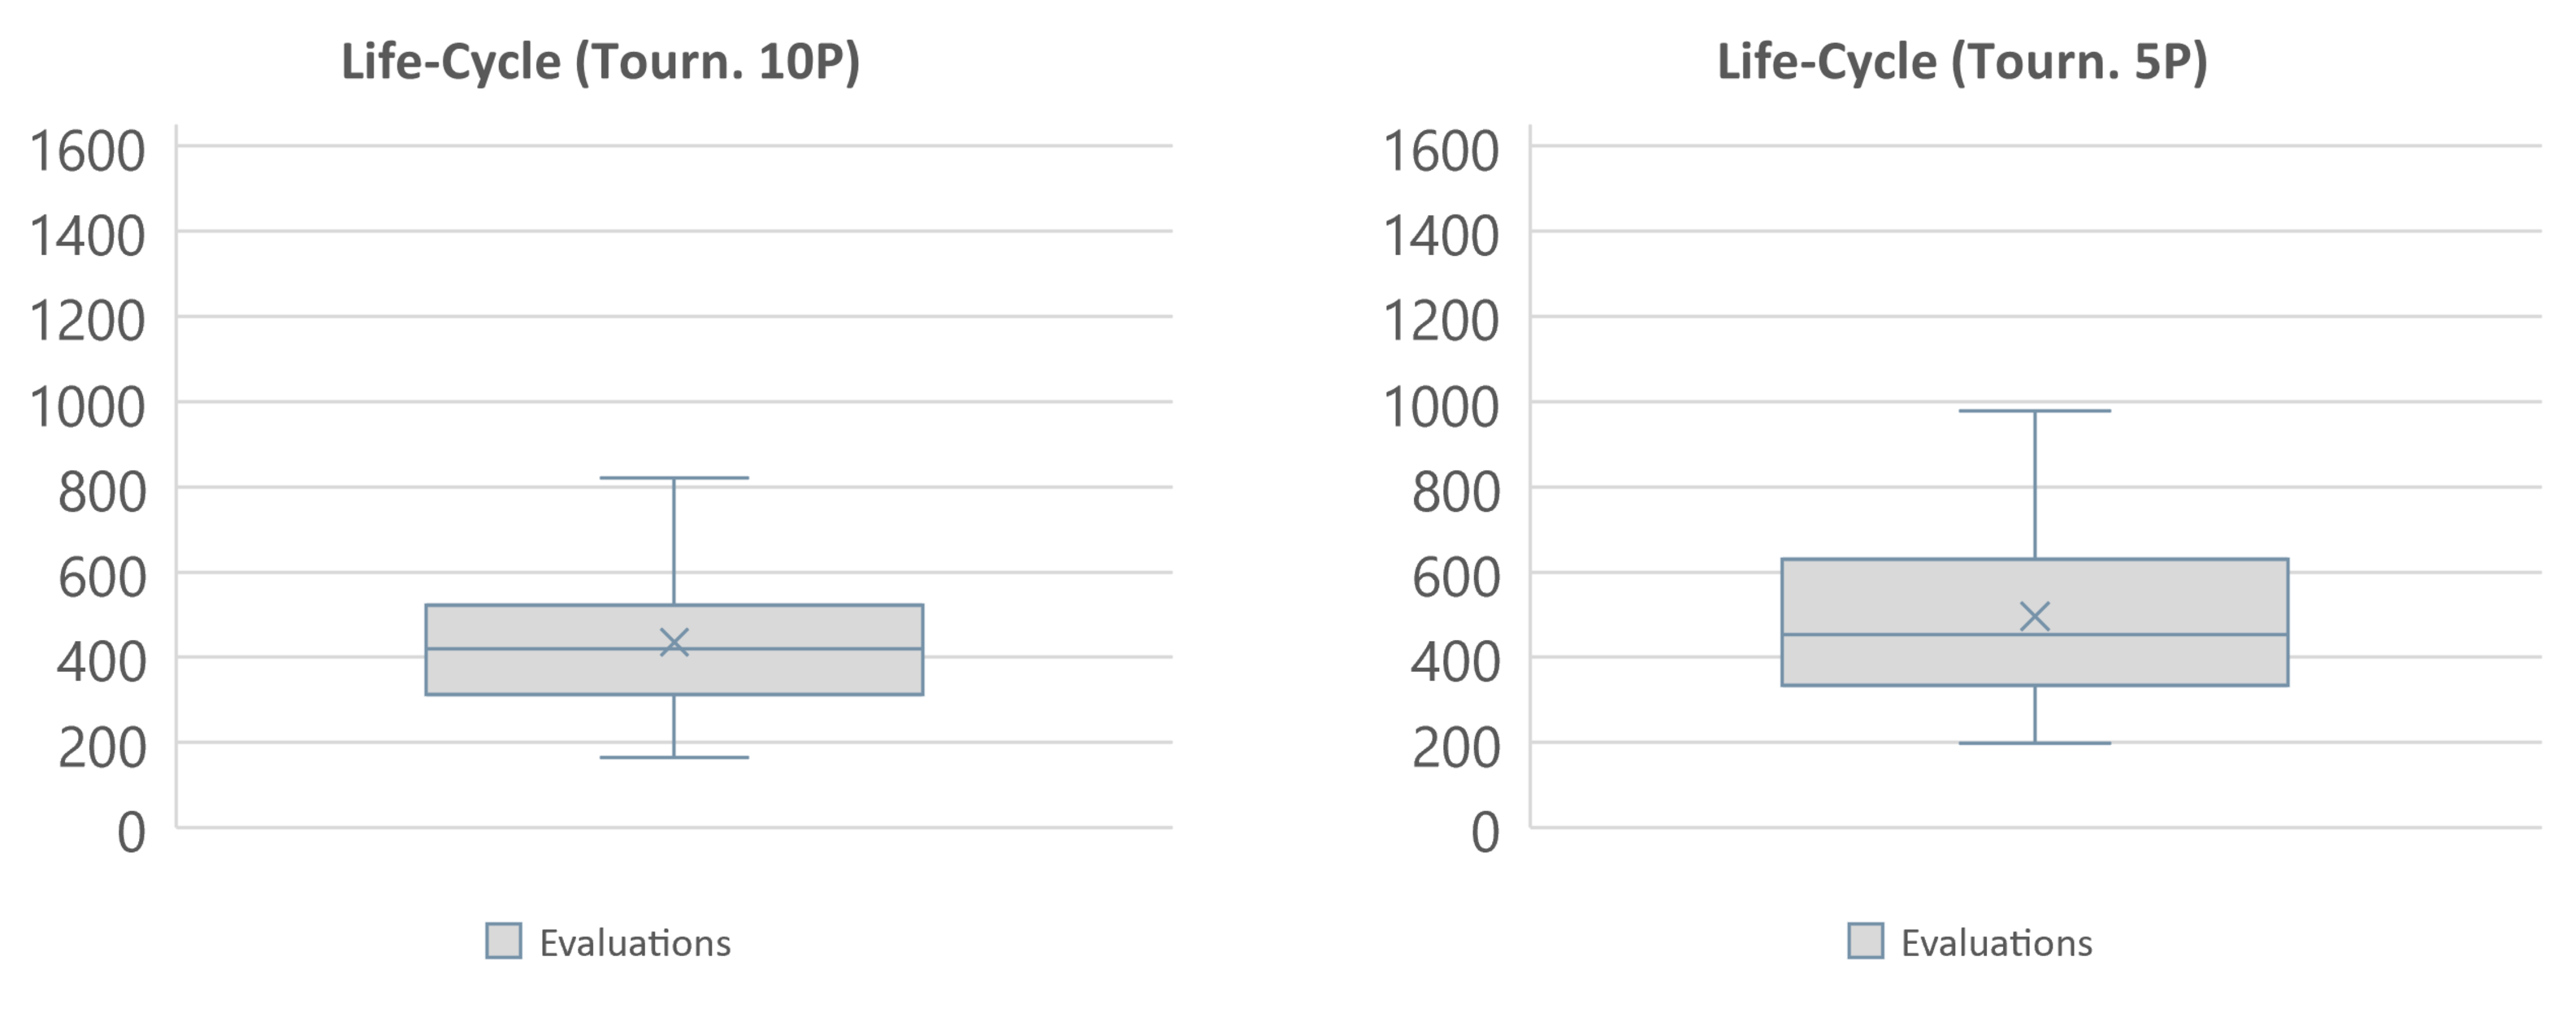
\includegraphics[width=\textwidth]{img/fig7_experiment02_chart.pdf}}
    \caption{Box and Whisker chart for the Experiment 2: Life-Cycle Tournament selection (10 versus 5 processes).} \label{fig.experiment2}
    \end{figure}


\subsubsection{Experiment 3} The goal of our third experiment was to follow and
study the behavior of the Life-Cycle algorithm that continued converging on the
solution. For this experiment, we remained using minimal delays (thousands of a
second magnitude). For this experiment, we only used tournament selection for
the reproduction, on the first configuration running the Life-Cycle on six
processes, two of whom was the Death process, versus the second configuration
where we reduced the processes to the minimum (five) but increasing the (Death)
goal approval range to 115. We show the summarized results in
Table~\ref{tab.experiment3}, and Figure~\ref{fig.experiment3} shows their Box
and Whisker chart.

\begin{table}[]
    \centering        
    \caption{Experiment 3 results, Life-Cycle Tournament: 6 processes (Death x2) versus 5 processes (80 to 115 goal).}\label{tab.experiment3}
    \begin{tabular}{|l|l|l|l|l|l|l|l|l|}
    \hline
    Run & \multicolumn{4}{l|}{LifeCycle (Tourn. 6P, Death x2)} & \multicolumn{4}{l|}{LifeCycle (Tourn. 5P, 80-115g)} \\ \hline
    1-60 & Last Gen. & Eval. & Time (sec) & Eval/sec & Last Gen. & Eval. & Time (sec) & Eval/sec \\ \hline
    Avg. & 8.0 & 483 & 0.846 & 571 & 6.4 & 384 & 0.695 & 553 \\ \hline
    \end{tabular}
    \end{table}

\begin{figure}
    \fbox{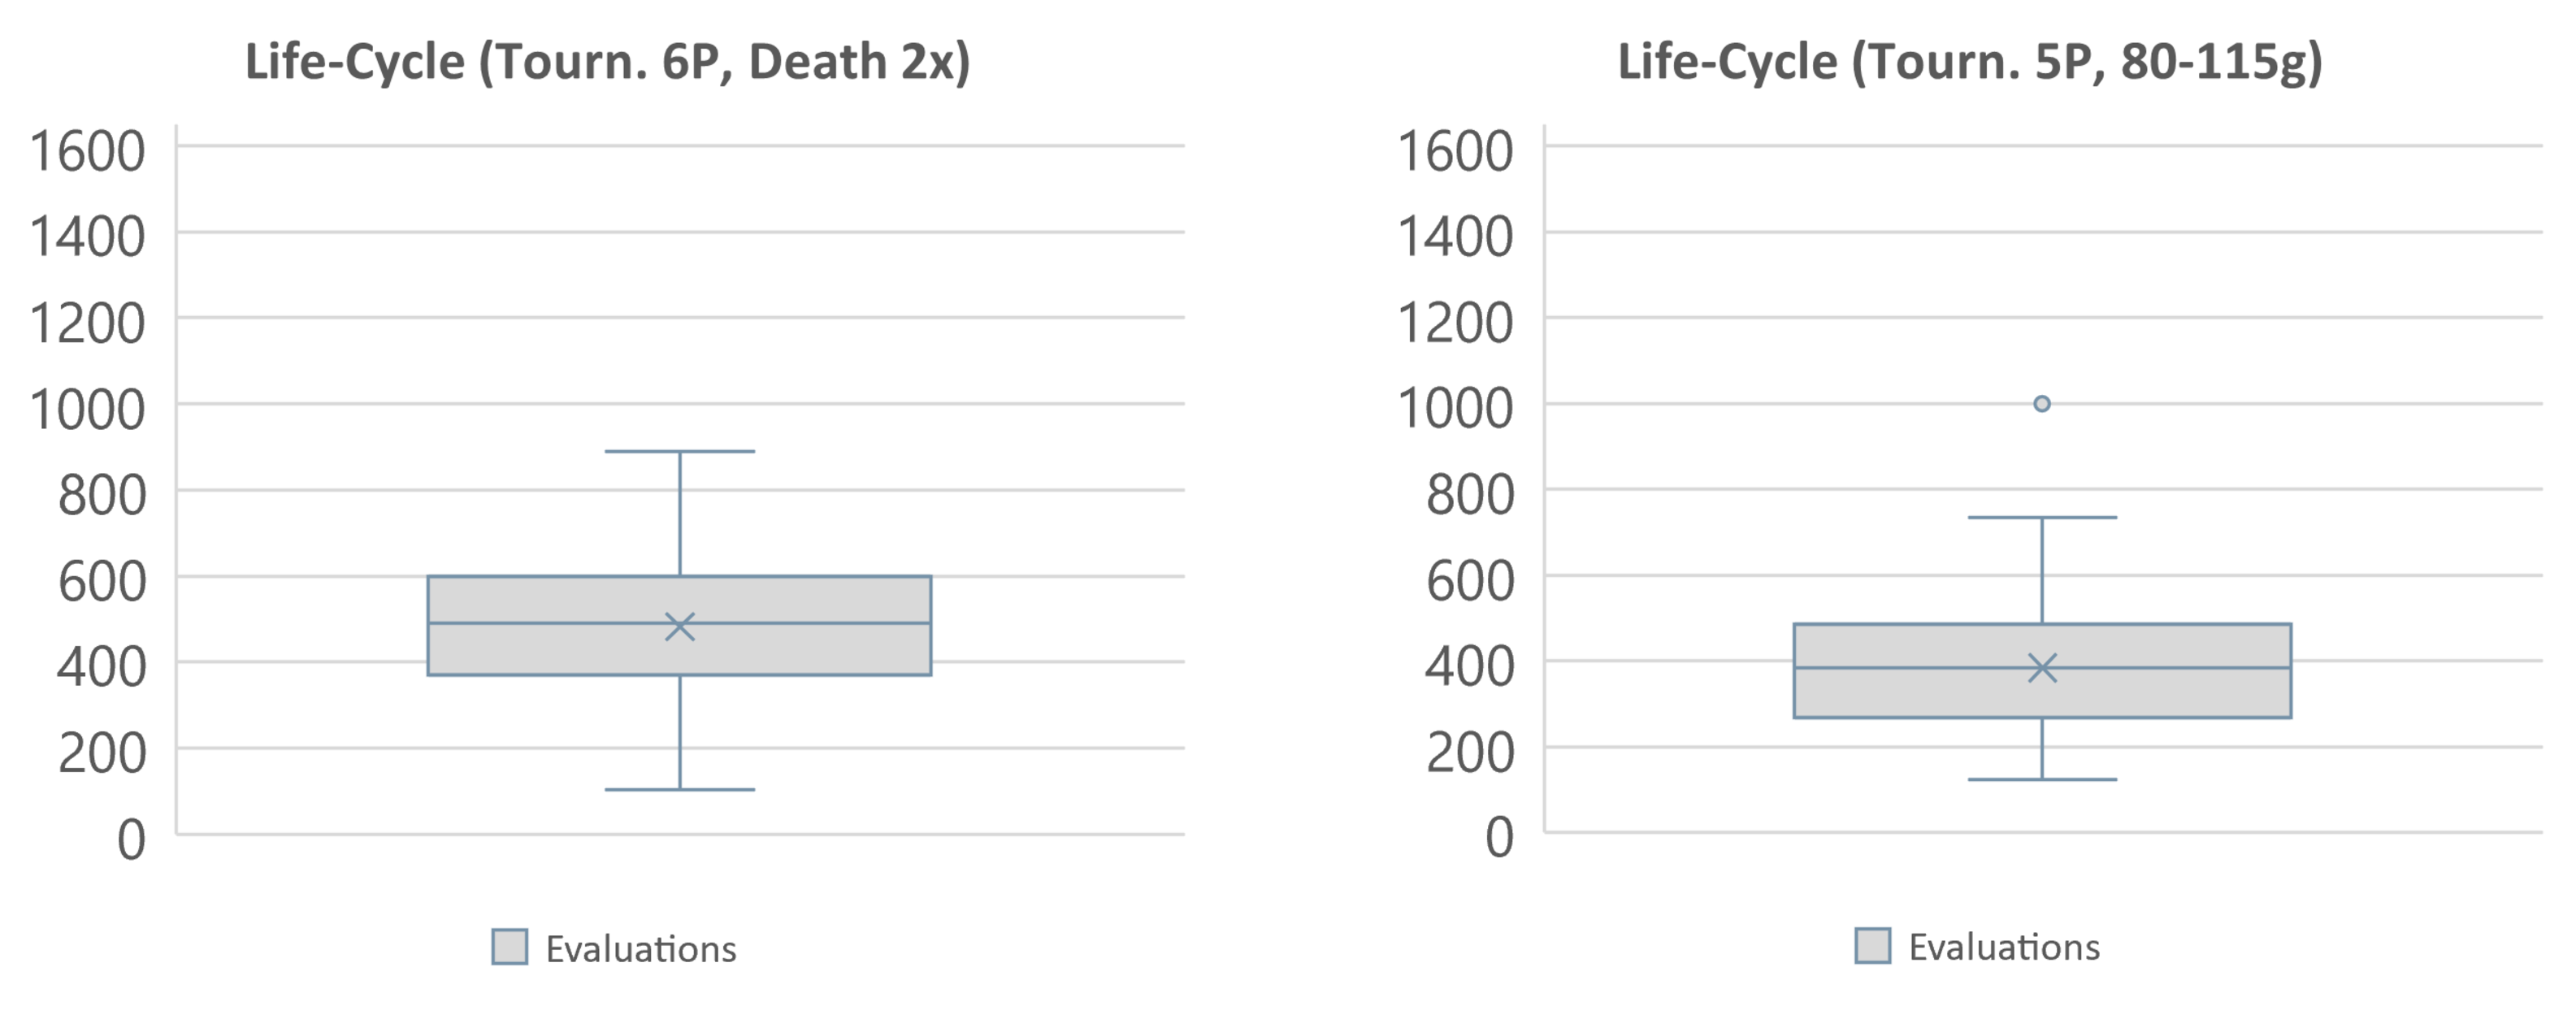
\includegraphics[width=\textwidth]{img/fig8_experiment03_chart.pdf}}
    \caption{Box and Whisker chart for the Experiment 3: Life-Cycle Tournament (6 processes double Death, versus 5 processes with an 80 to 115 goal approval).} \label{fig.experiment3}
    \end{figure}


\subsubsection{Experiment 4} The goal of our fourth and last experiment was to
follow and study the behavior of the Life-Cycle algorithm that continued
converging on the solution. For this experiment, we remained using minimal
delays (thousands of a second magnitude). For this experiment, we compared the
OneMax DEAP implementation versus the Life-Cycle algorithm, only using
tournament selection for the reproduction, with the Life-Cycle configuration
running on the minimum (five) processes but increasing the (Death) goal
approval range to 125. We show the summarized results in
Table~\ref{tab.experiment4}, and Figure~\ref{fig.experiment4} shows their Box
and Whisker chart.

\begin{table}[]
    \centering        
    \caption{Experiment 4 results, OneMax DEAP versus Life-Cycle Tournament: 5 processes (80 to 125 goal).}\label{tab.experiment4}
    \begin{tabular}{|l|l|l|l|l|l|l|l|l|}
    \hline
    Run & \multicolumn{4}{l|}{OneMax DEAP} & \multicolumn{4}{l|}{Life-Cycle (Tourn. 5P, 80-125g)} \\ \hline
    1-60 & Last Gen. & Eval. & Time (sec) & Eval/sec & Last Gen. & Eval. & Time (sec) & Eval/sec \\ \hline
    Avg. & 6.5 & 391 & 0.036 & 10,836 & 6.3 & 377 & 0.678 & 556 \\ \hline
    \end{tabular}
    \end{table}

\begin{figure}
    \fbox{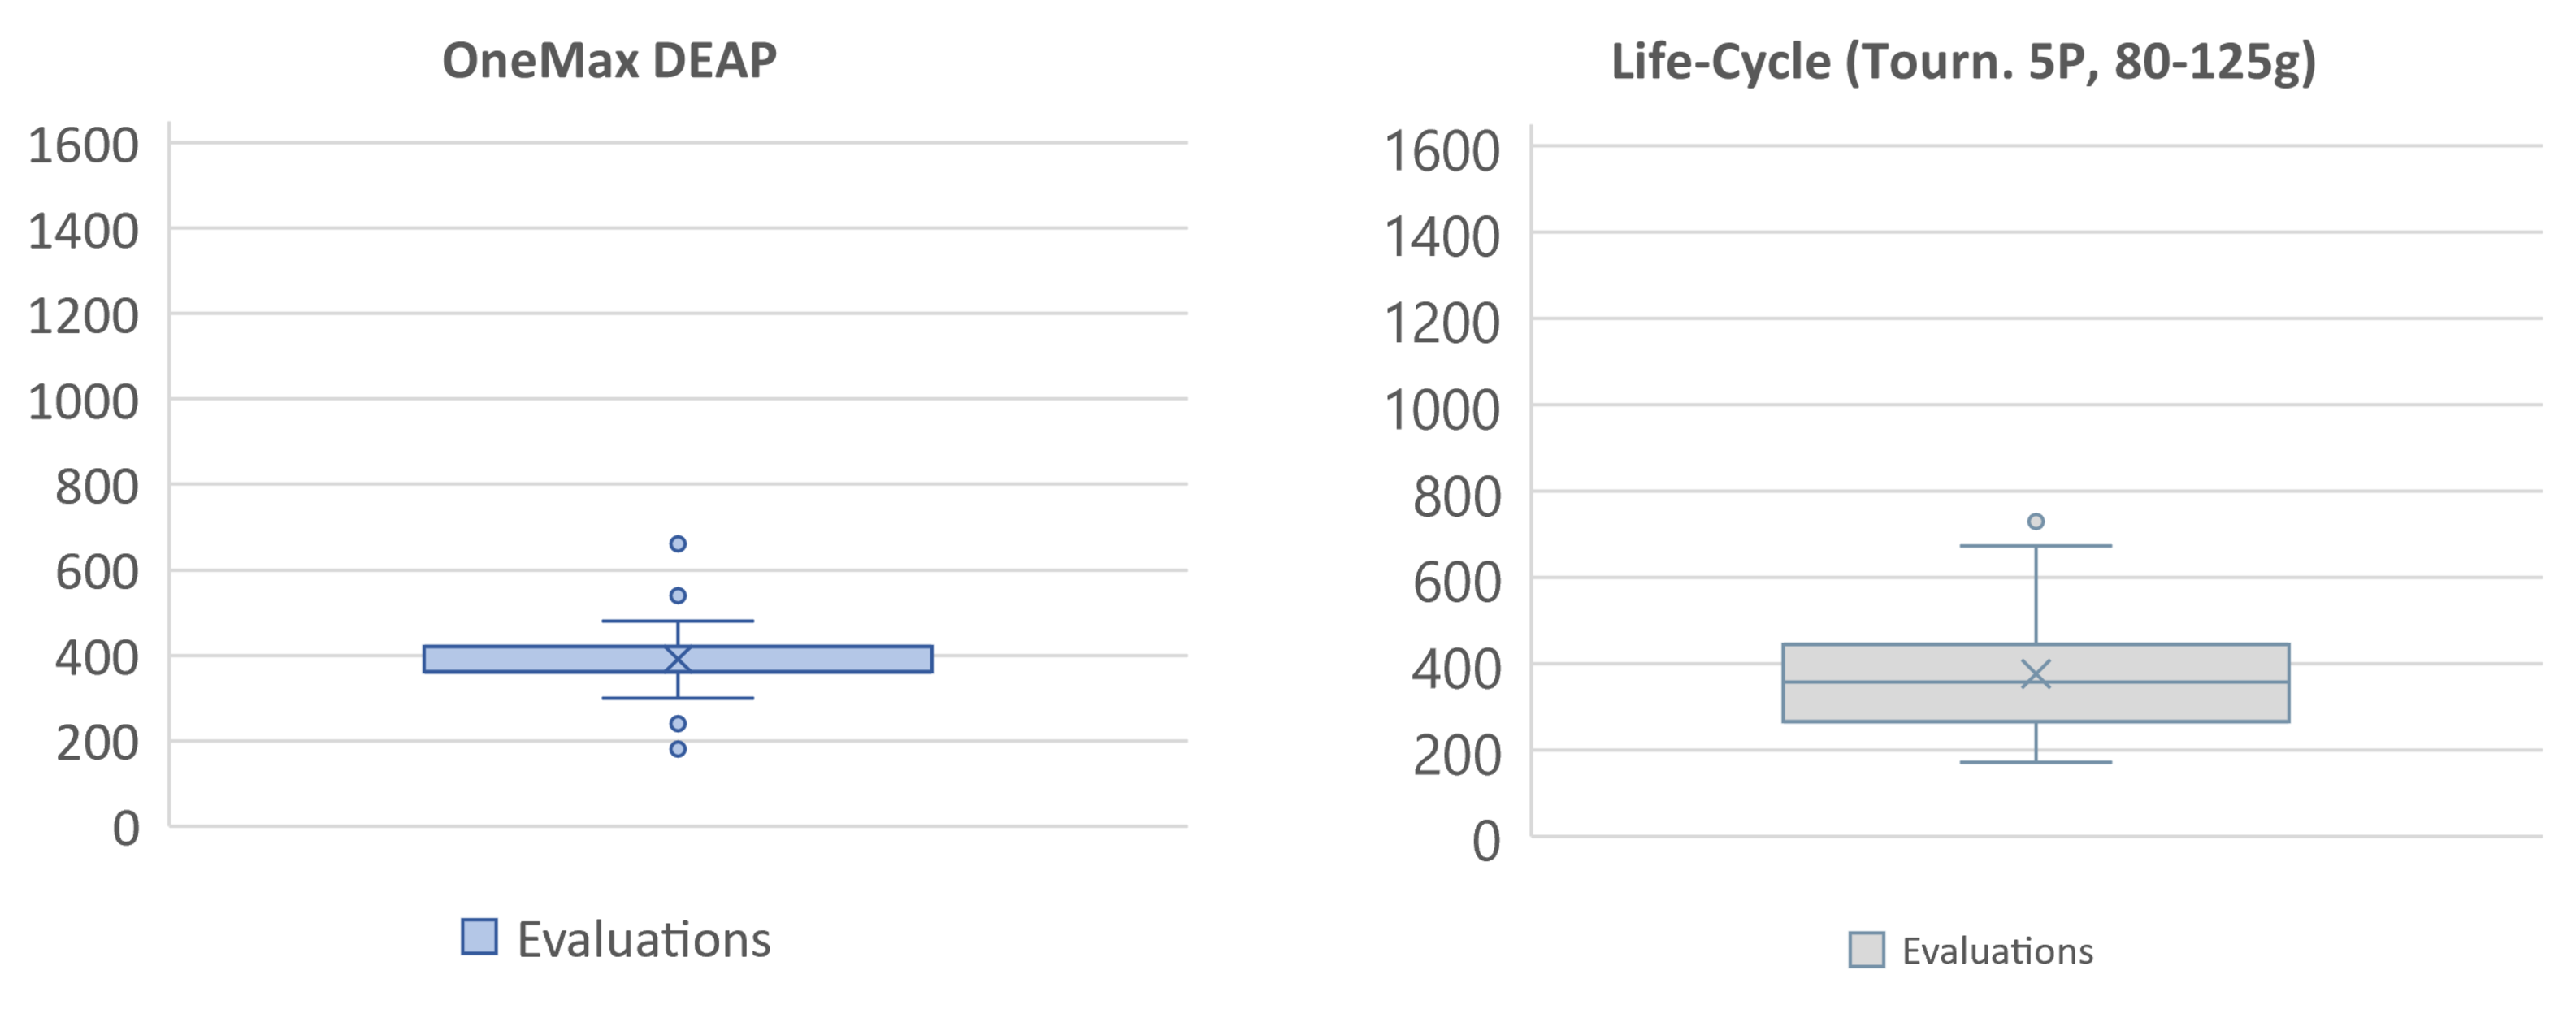
\includegraphics[width=\textwidth]{img/fig9_experiment4_chart.pdf}}
    \caption{Box and Whisker chart for the Experiment 4: OneMax DEAP versus Life-Cycle Tournament (5 processes with an 80 to 125 goal approval).} \label{fig.experiment4}
    \end{figure}




\begin{acknowledgement}
    This paper has been supported in part by projects DeepBio (TIN2017--85727--C4--2--P) and TecNM Project 11356.21\@.
\end{acknowledgement}

% ---- Bibliography ----
% BibTeX users should specify bibliography style 'splncs04'.
% References will then be sorted and formatted in the correct style.
%
\bibliographystyle{splncs04}
\bibliography{bib/bibliografia.bib}

\end{document}
